\chapter{Feature selection and importance: Biomedical analysis}


\section{Data}

The dataset contains anonymized biomedical data and is composed of a binary target variable and unknown variables.

\begin{remark}
    In reality, this dataset contains real-world examples. Features have been anonymized for the purpose of feature analysis.
\end{remark}


\subsection{Preliminary analysis}

\begin{description}
    \item[Data distribution]
        There are both categorical and numerical features.
        \begin{figure}[H]
            \centering
            \begin{subfigure}{0.75\linewidth}
                \centering
                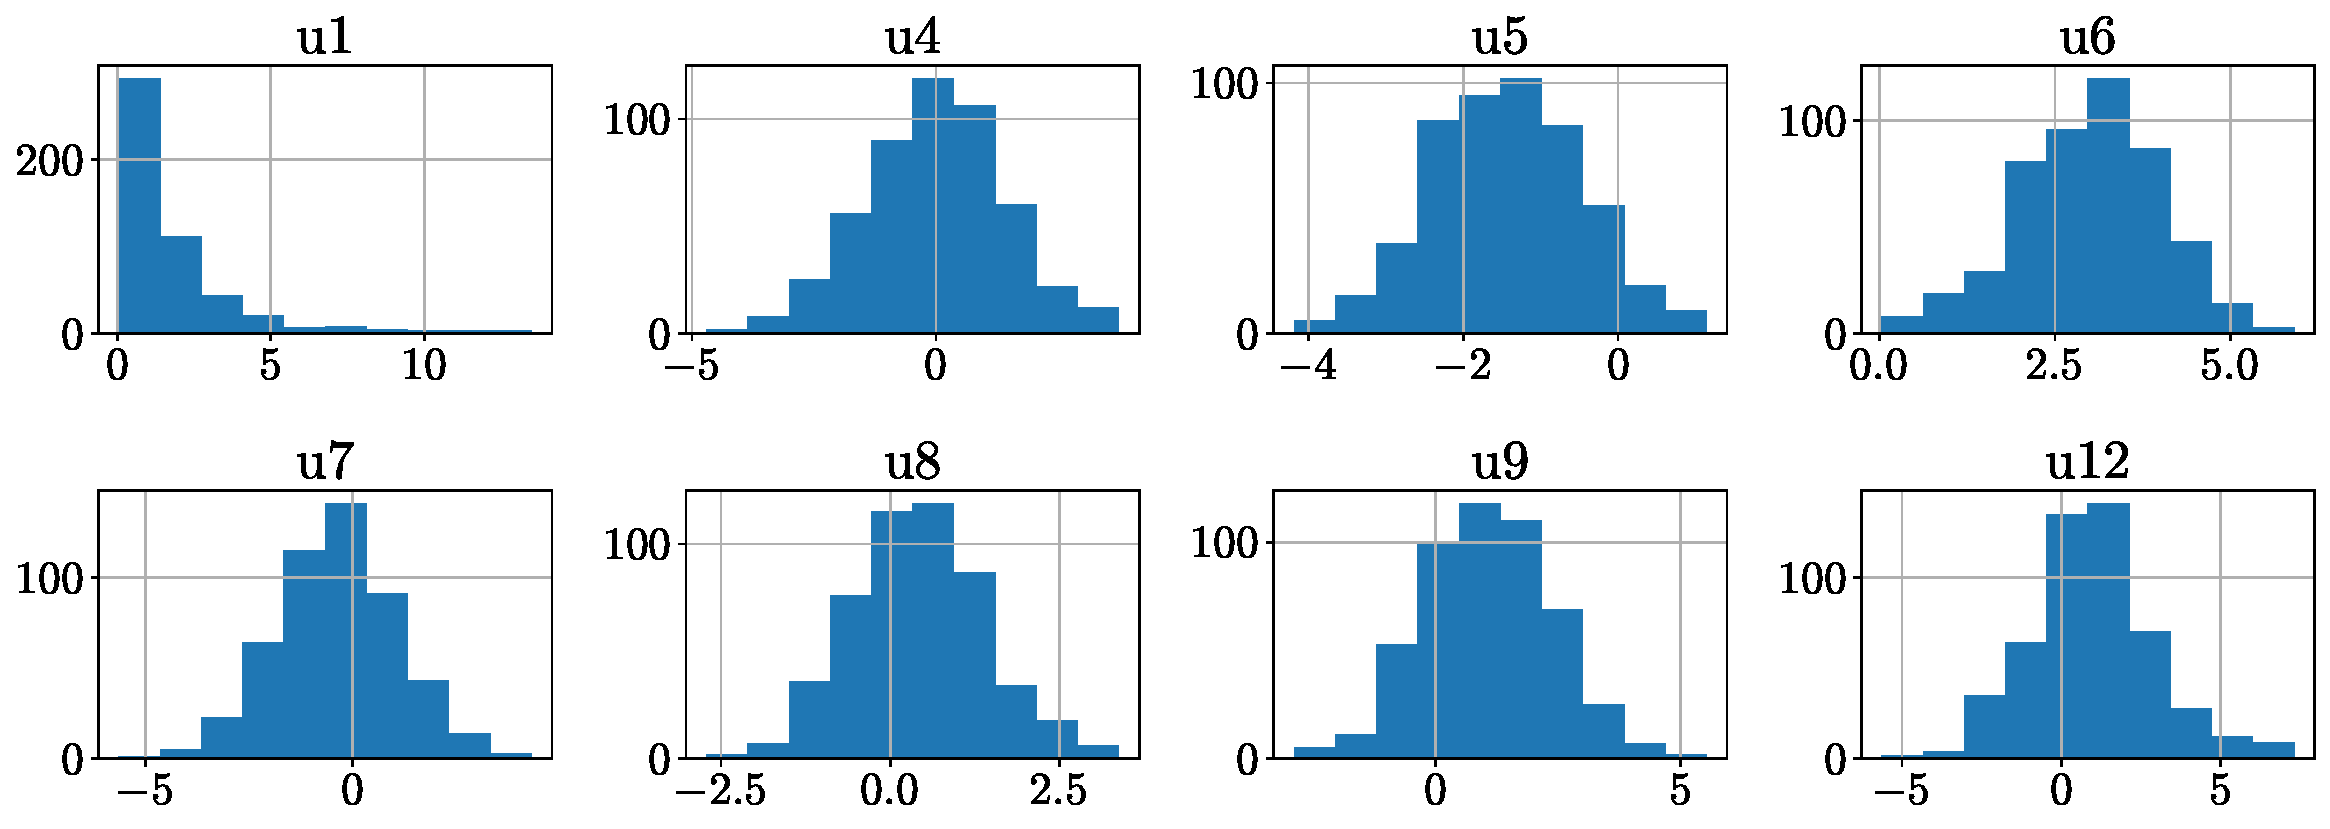
\includegraphics[width=\linewidth]{./img/_biomed_numeric_distr.pdf}
                \caption{Numerical features}
            \end{subfigure}
            \begin{subfigure}{0.75\linewidth}
                \centering
                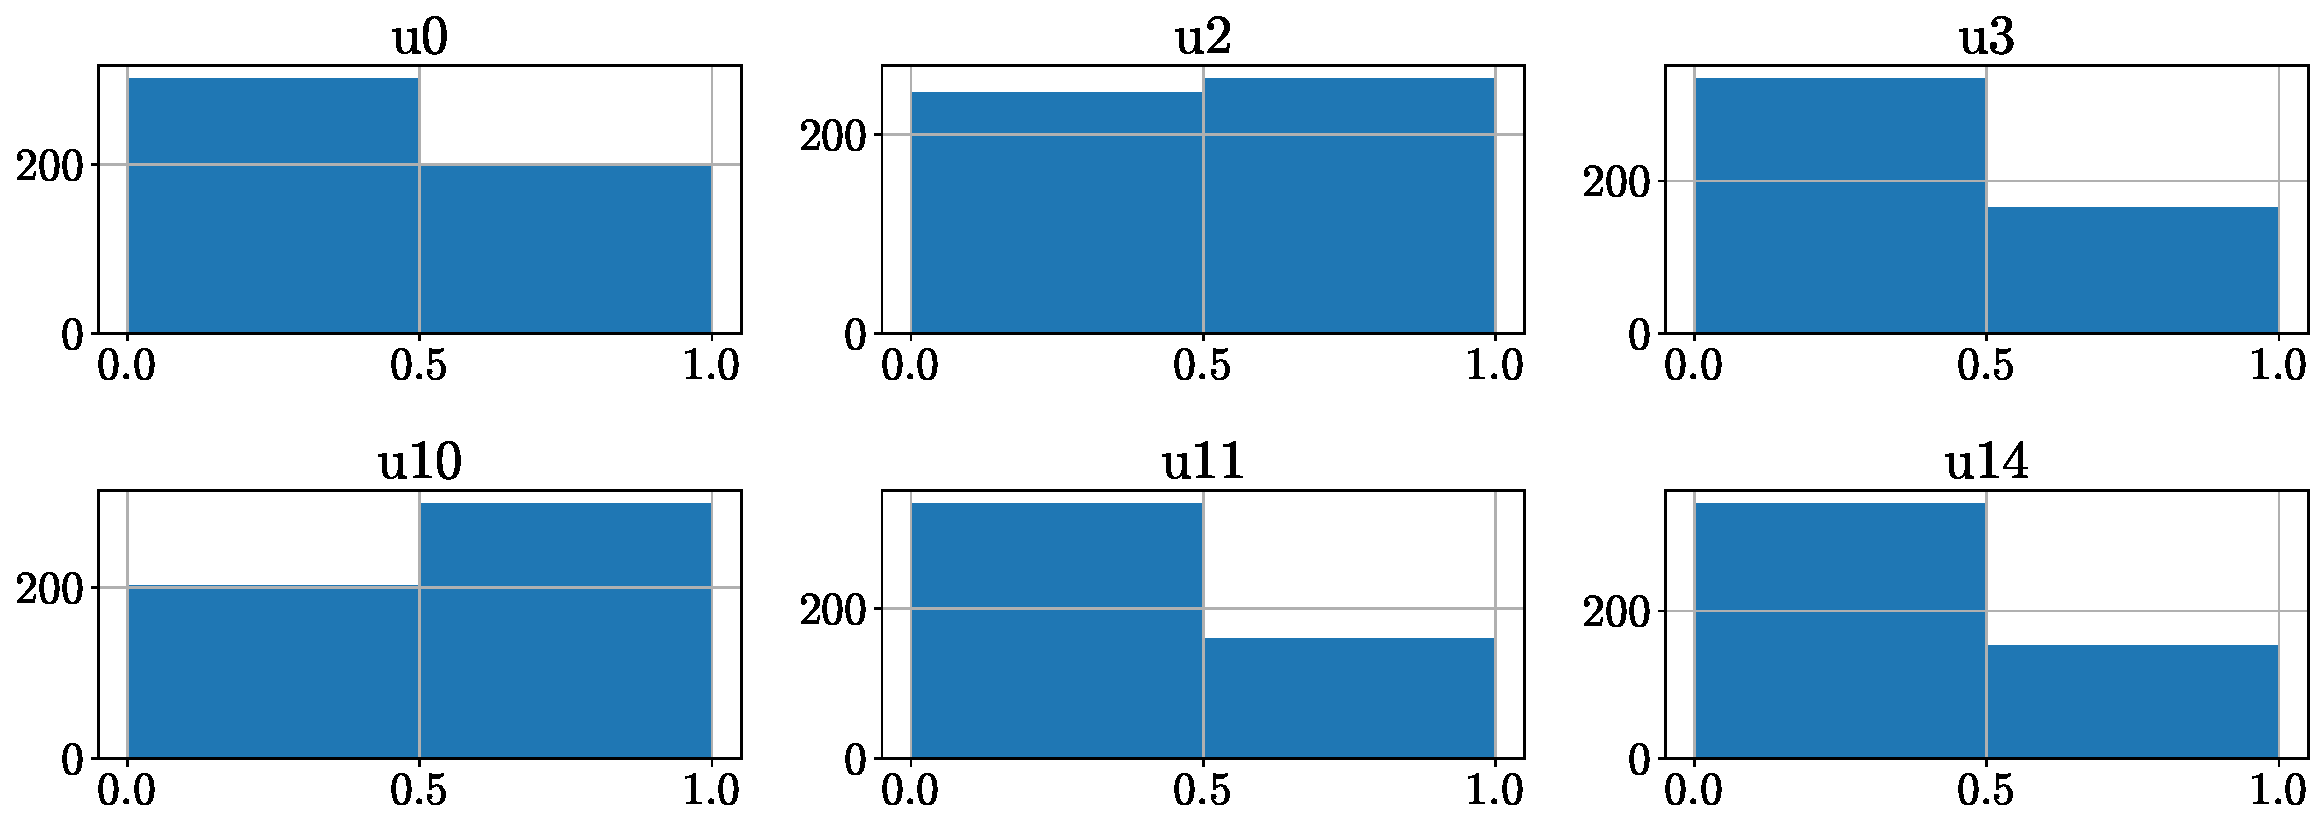
\includegraphics[width=\linewidth]{./img/_biomed_categ_distr.pdf}
                \caption{Categorical features}
            \end{subfigure}
            \begin{subfigure}{0.2\linewidth}
                \centering
                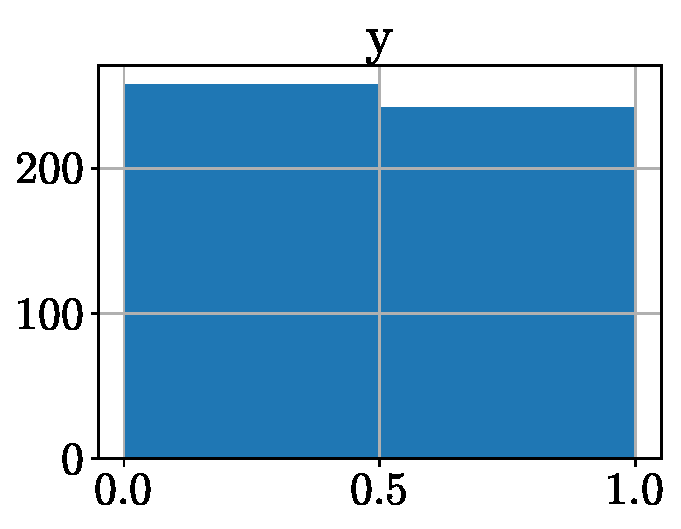
\includegraphics[width=\linewidth]{./img/_biomed_target_distr.pdf}
                \caption{Target}
            \end{subfigure}
            \caption{Distribution of the dataset}
        \end{figure}

    \item[Univariate dependencies]
        Determine the fraction of examples with target $Y=1$ (i.e., likelihood that a feature has a specific value while the target is $1$).

        \begin{figure}[H]
            \centering
            \begin{subfigure}{0.75\linewidth}
                \centering
                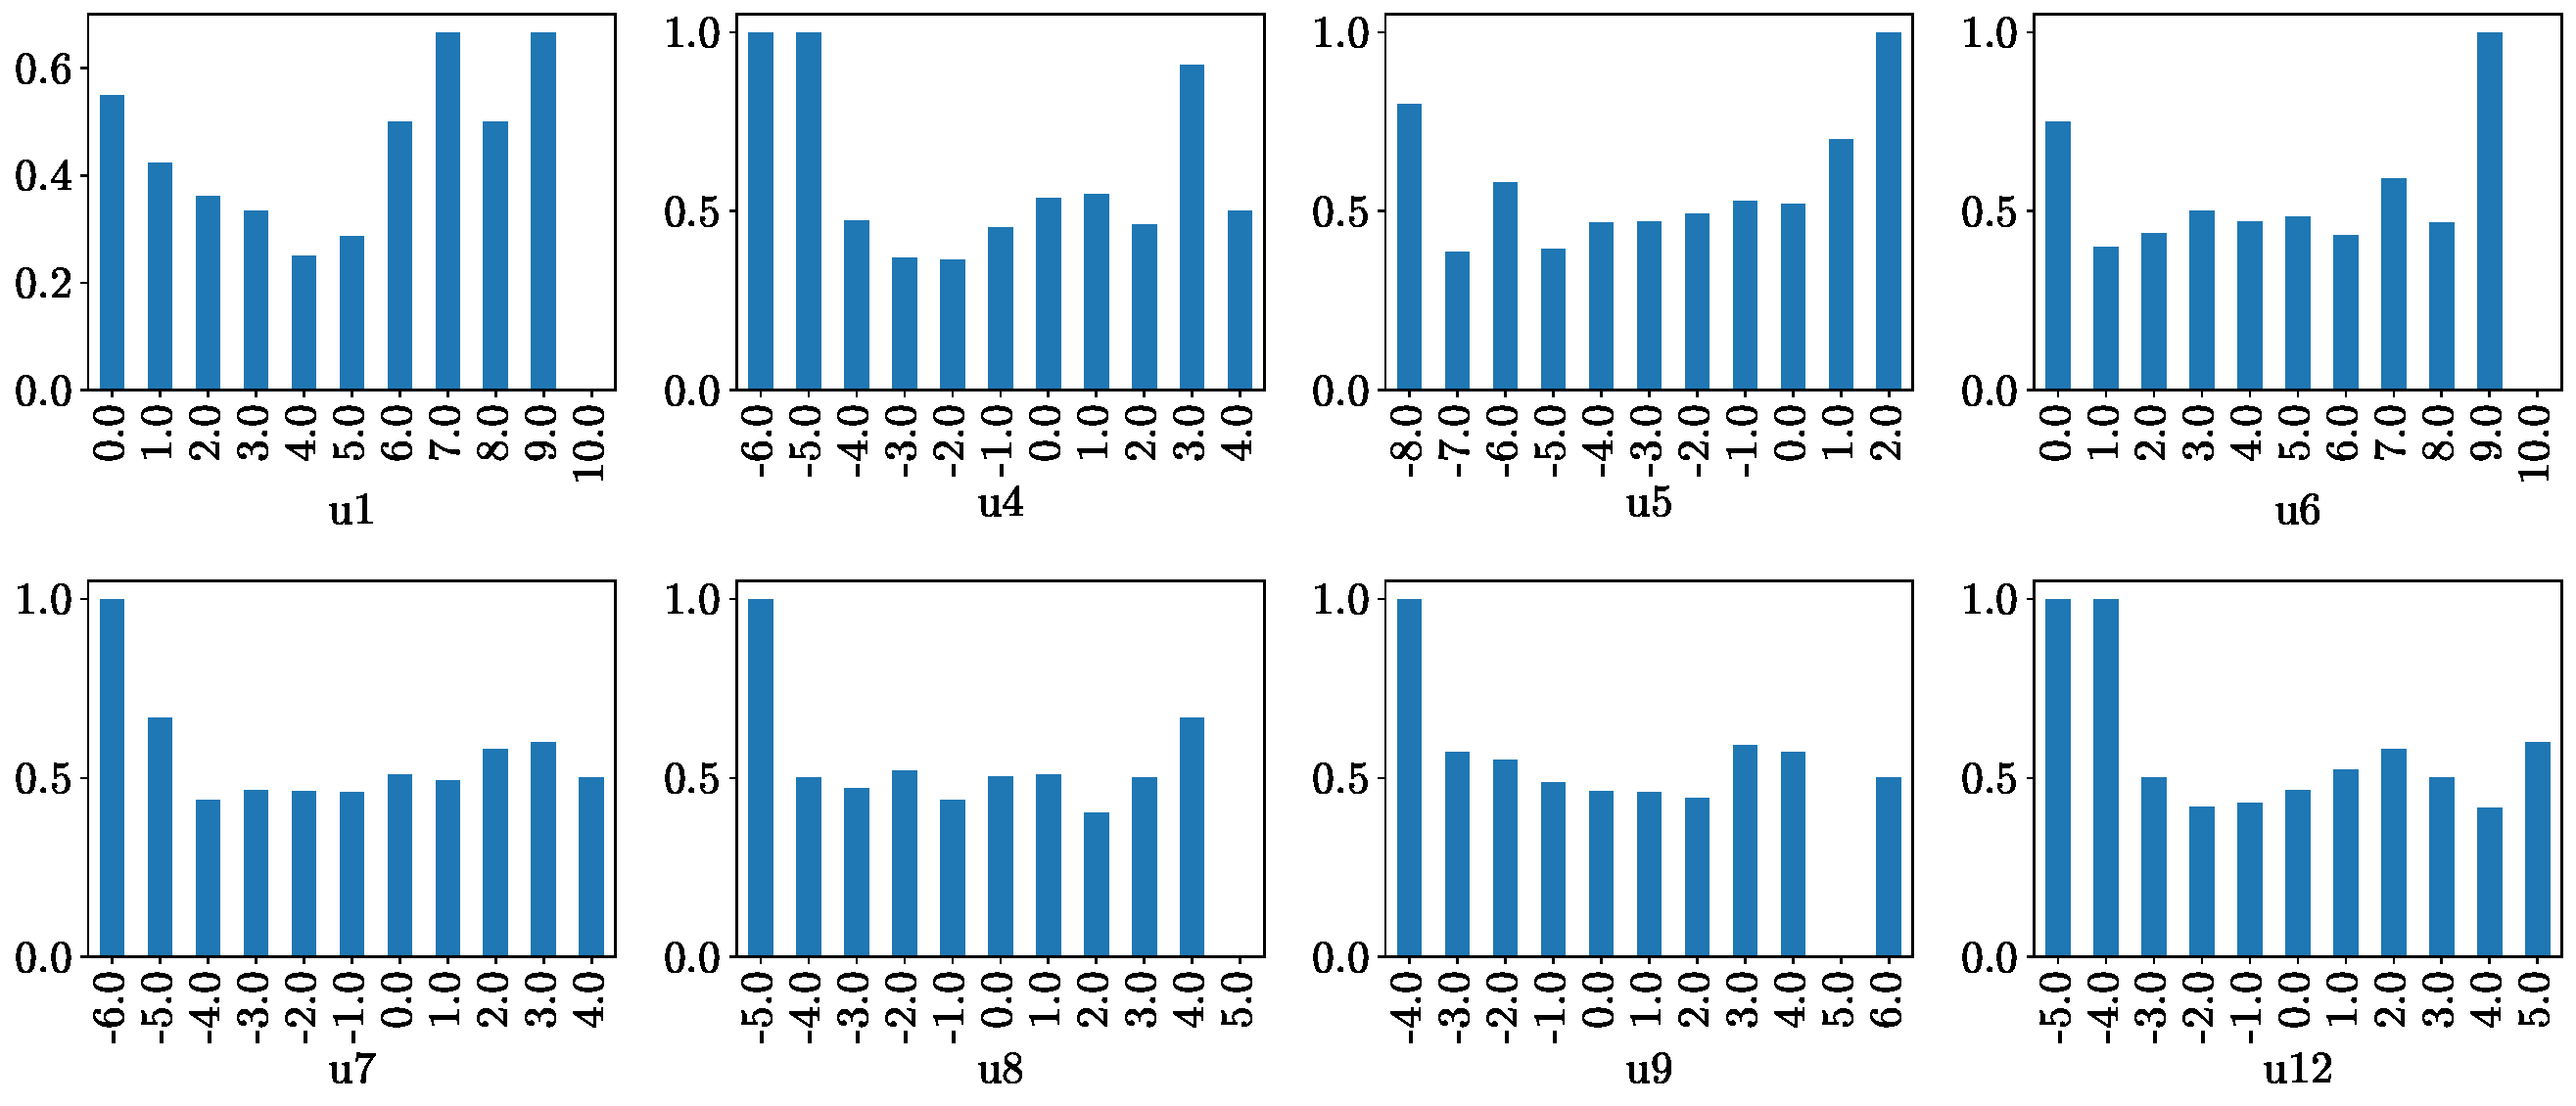
\includegraphics[width=\linewidth]{./img/_biomed_target_num_distr.pdf}
                \caption{Numerical features}
            \end{subfigure}
            \begin{subfigure}{0.75\linewidth}
                \centering
                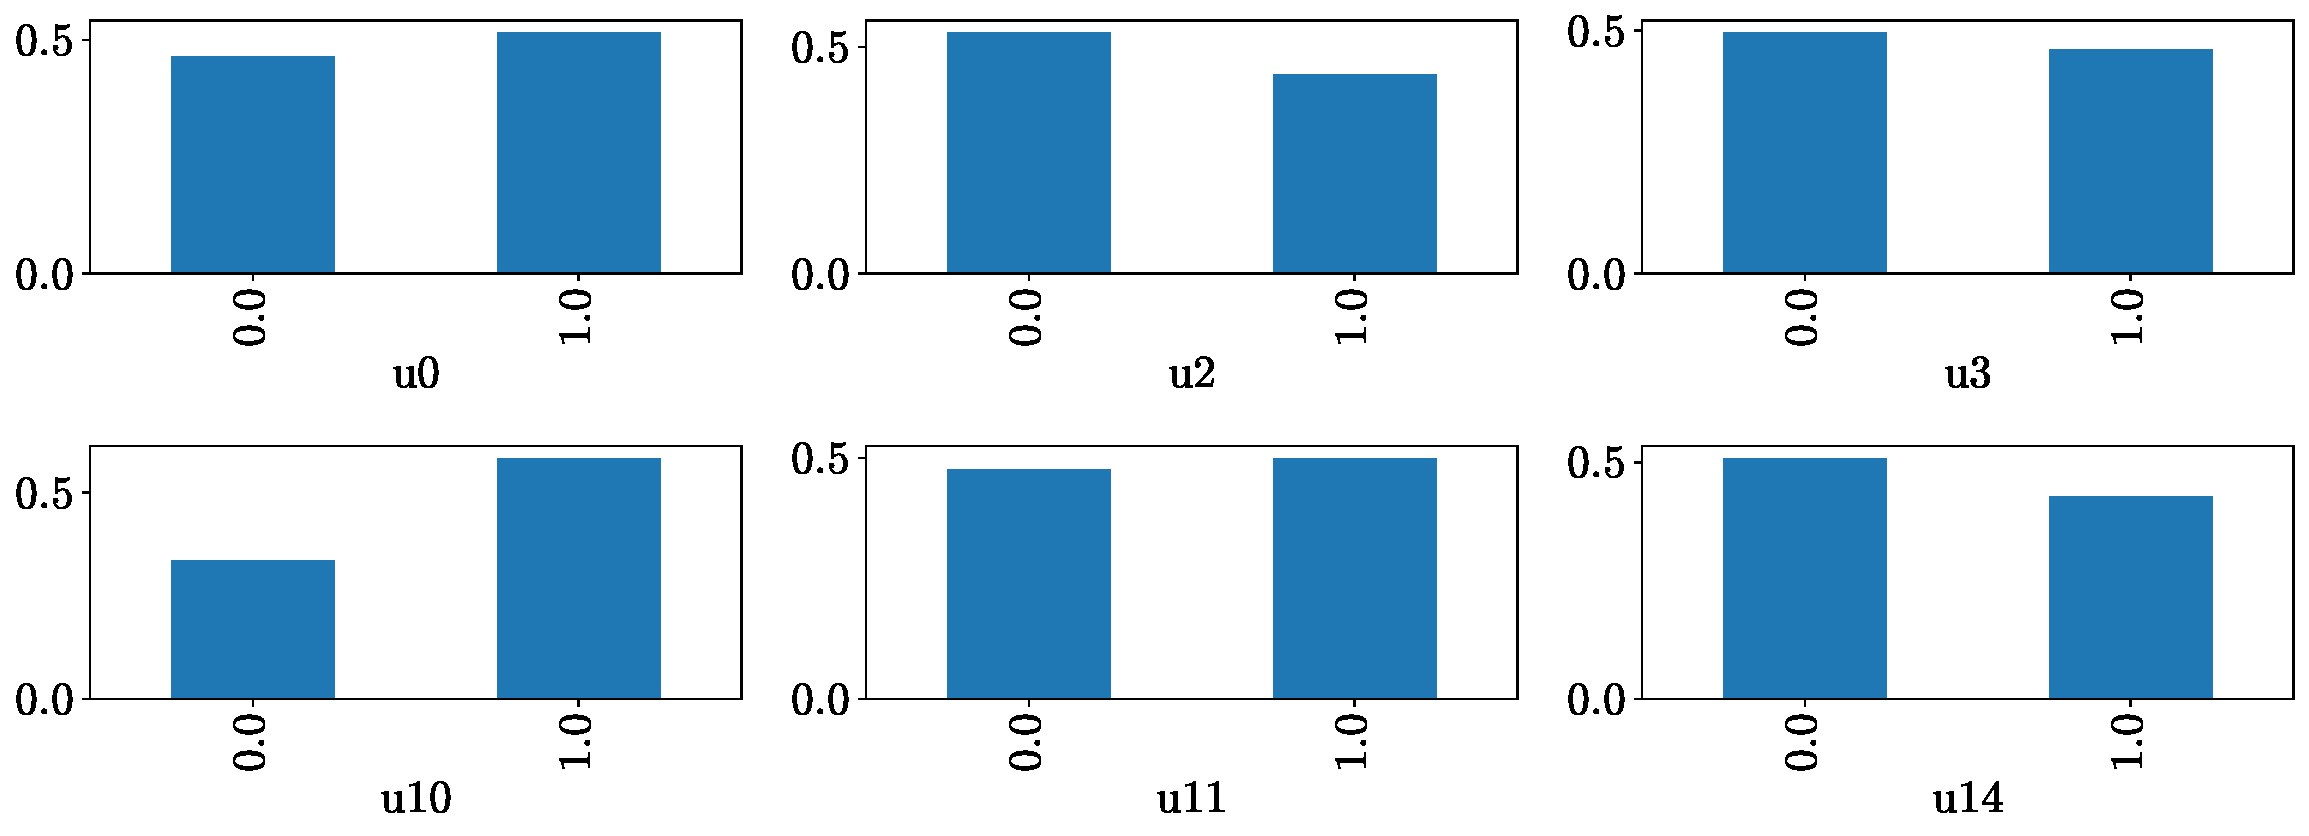
\includegraphics[width=\linewidth]{./img/_biomed_target_categ_distr.pdf}
                \caption{Categorical features}
            \end{subfigure}
            \caption{Univariate dependencies with $Y=1$}
        \end{figure}

    \item[Linear correlation]
        Determine the Pearson's correlation between variables.

        \begin{figure}[H]
            \centering
            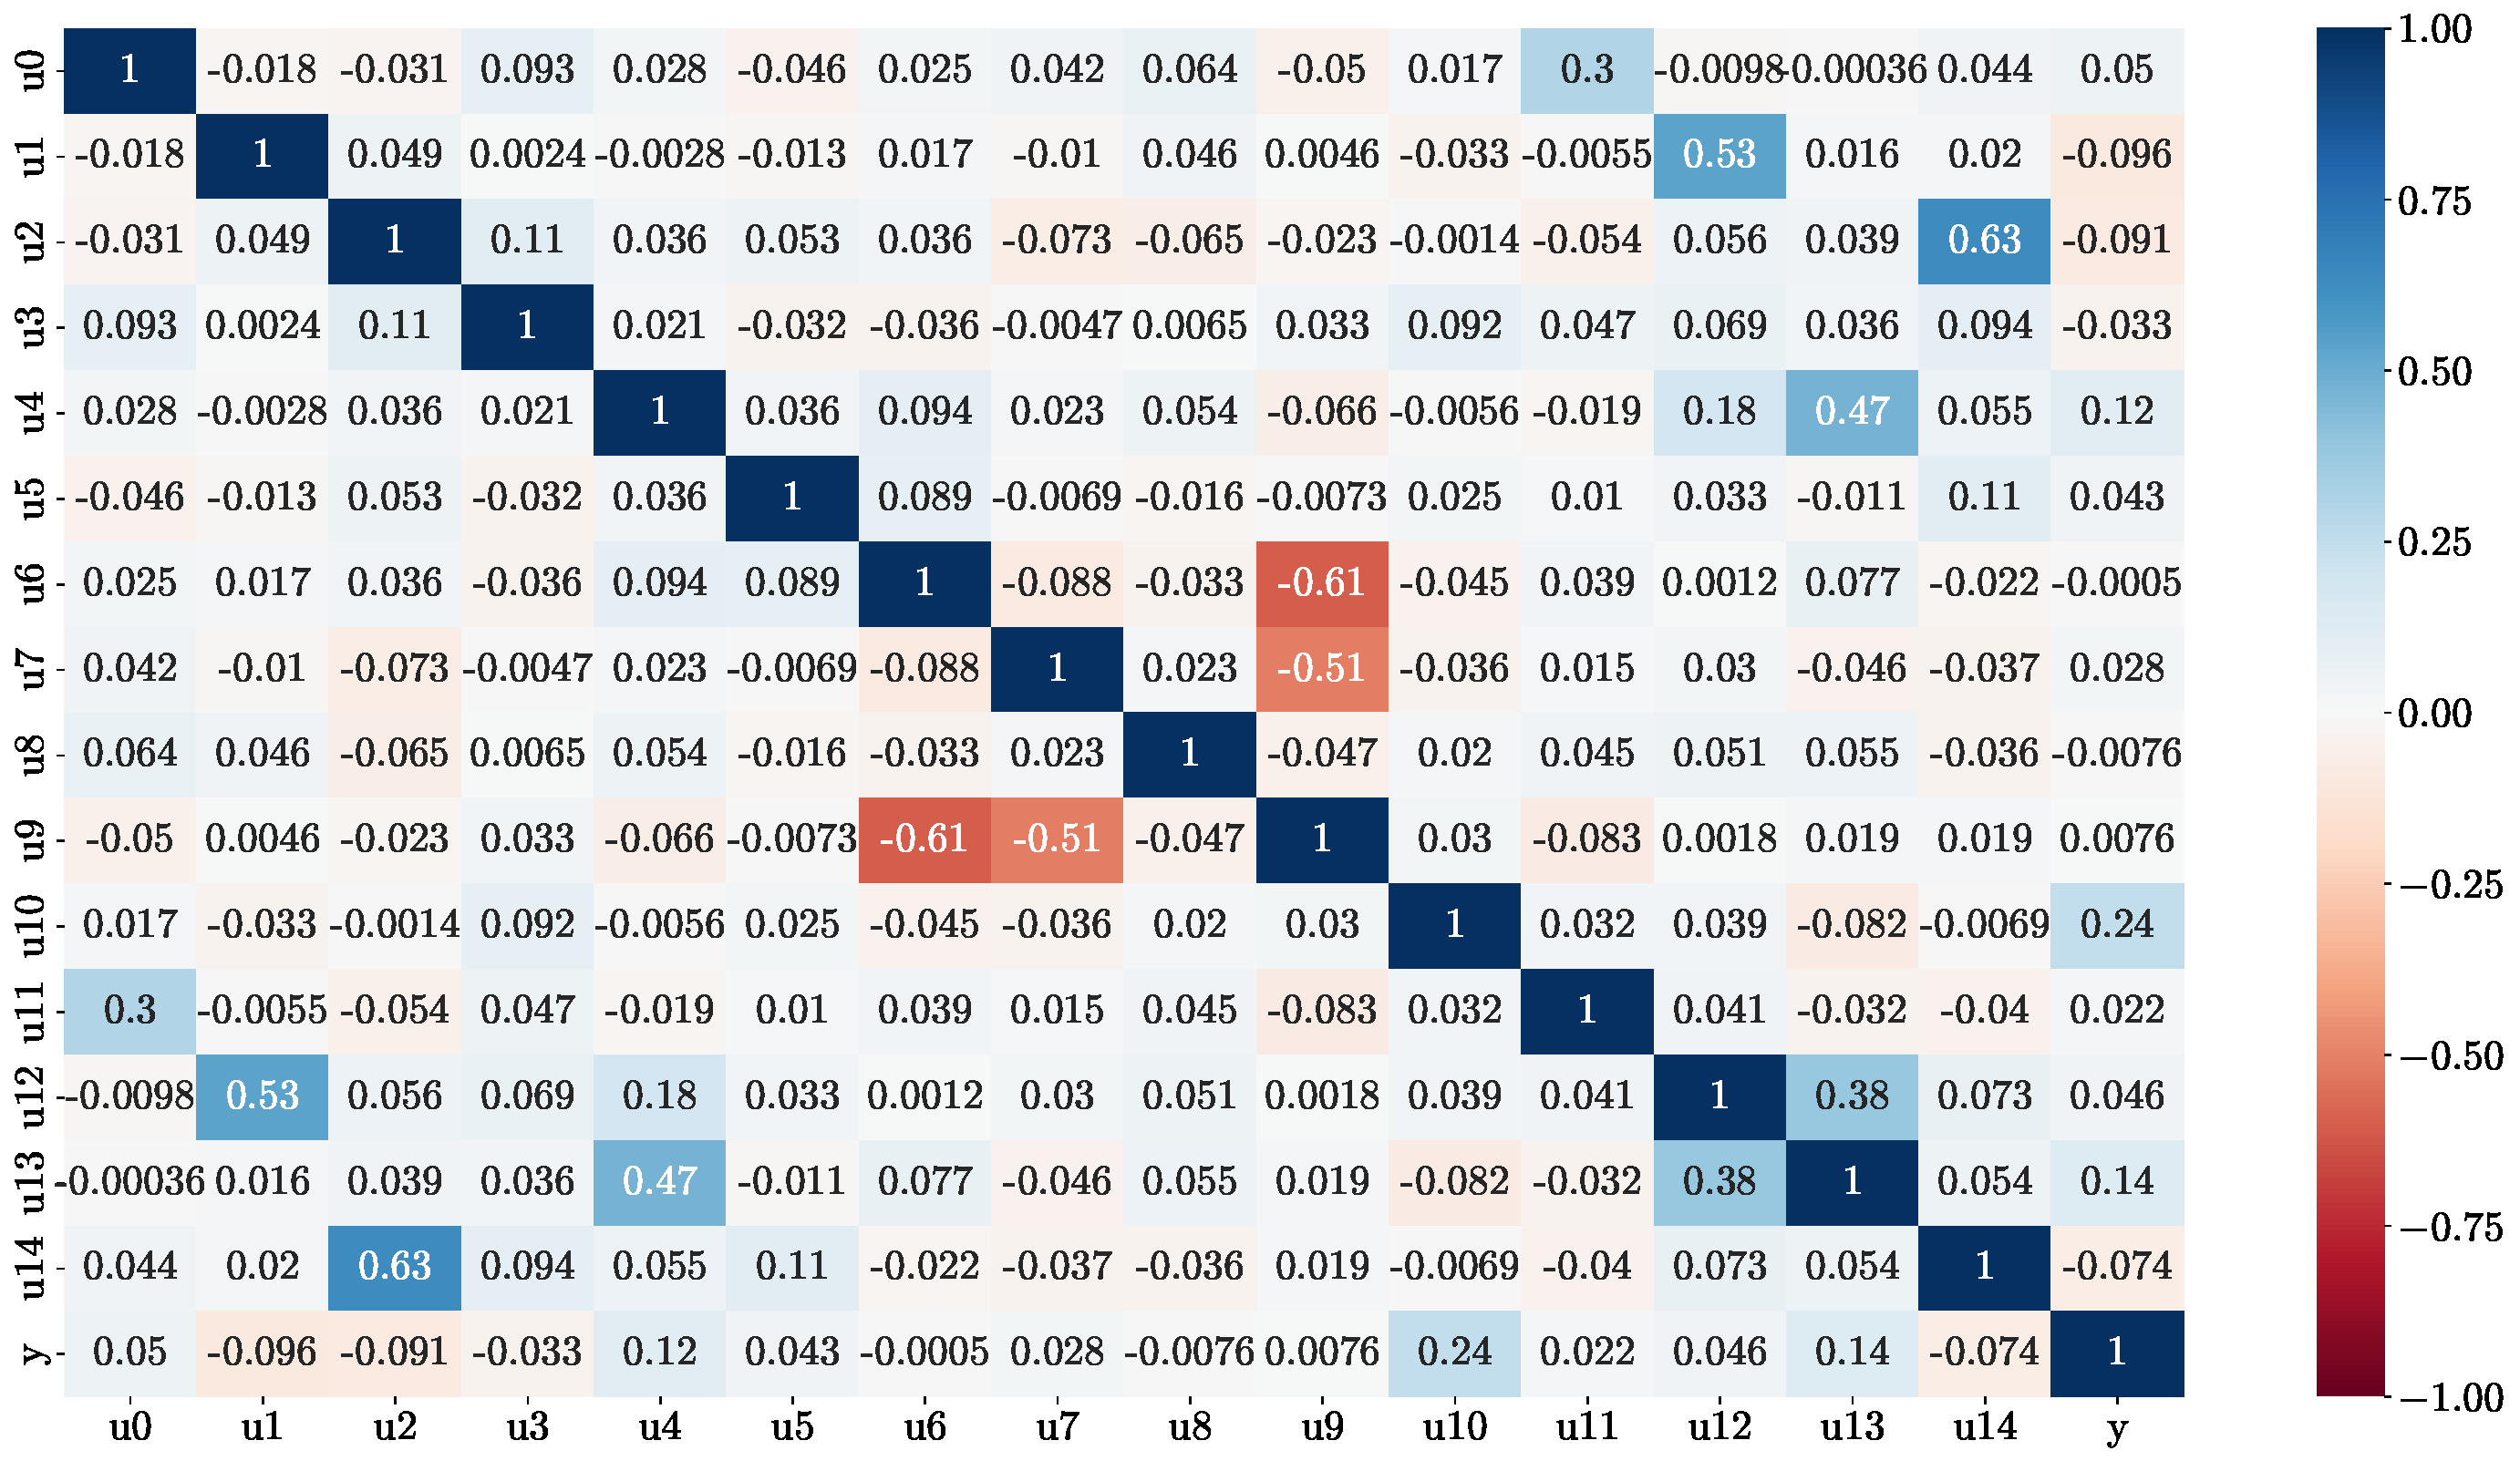
\includegraphics[width=0.8\linewidth]{./img/_biomed_corr_matrix.pdf}
        \end{figure}
\end{description}



\section{Approaches}


\subsection{Linear model}

\begin{description}
    \item[Linear model for explanation] \marginnote{Linear model for explanation}
        Use a linear model (logistic regression in this case) as a proxy to explain the features.

        \begin{remark}
            Preventing overfitting is important as the model has to generalize well. L1 regularization ($\alpha \Vert \vec{\theta} \Vert_1$) can help by:
            \begin{itemize}
                \item Preventing overfitting.
                \item Sparsifying the coefficients (i.e., make them mostly close to $0$). The hyperparameter $\alpha$ controls this behavior.
                    \begin{example}
                        Consider the case of MSE with L1 regularization.
                        The gradient of L1 is never $0$ and is upper-bounded whereas the gradient of MSE can be $0$ and can go to $\infty$. This produces the following phenomenon:
                        \begin{itemize}
                            \item When close to $0$, the slope of $\nabla\texttt{MSE}$ is larger and outweighs $\nabla\texttt{L1}$, making updates follow MSE.
                            \item When moving away from $0$, $\nabla\texttt{MSE}$ becomes smaller up to a point where it balances with $\nabla\texttt{L1}$. At this point, updating that parameter does not improve the loss anymore.
                        \end{itemize}

                        \begin{figure}[H]
                            \centering
                            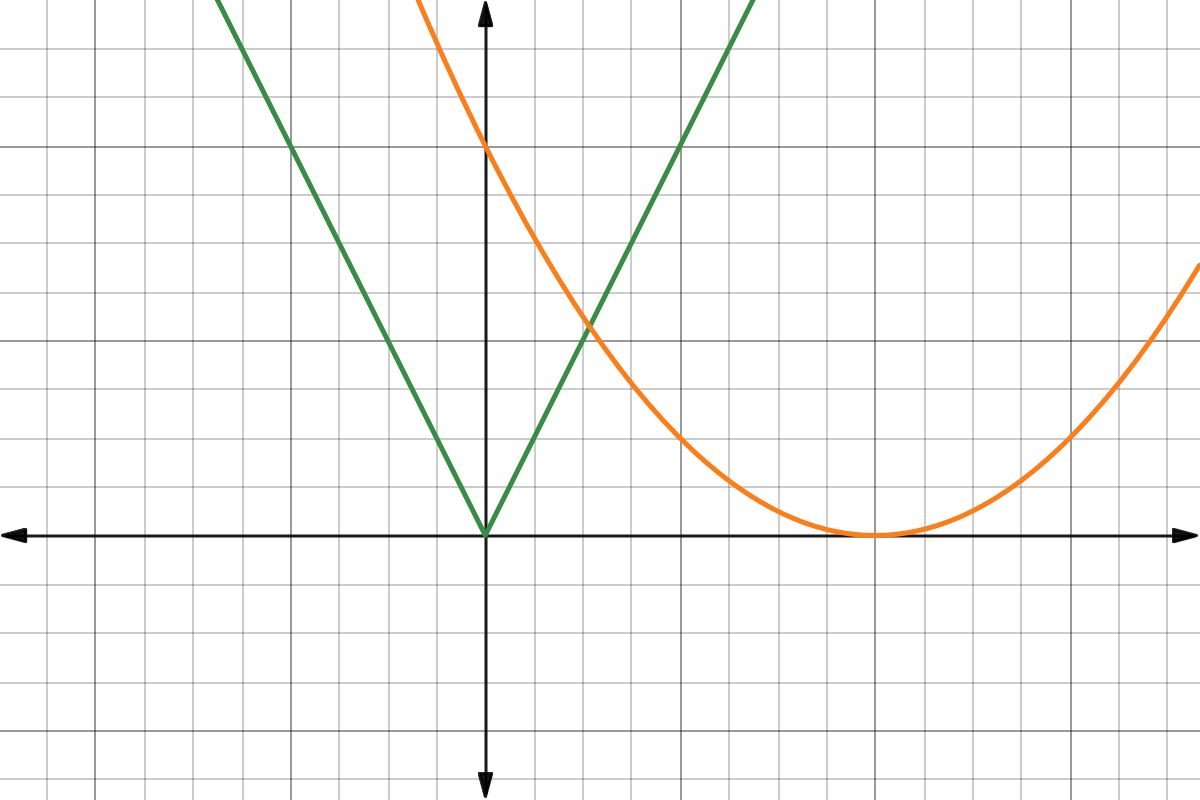
\includegraphics[width=0.4\linewidth]{./img/mse_l1.png}
                            \caption{MSE (orange) and L1 (green)}
                        \end{figure}
                    \end{example}
            \end{itemize}
        \end{remark}

        \begin{remark}
            ROC-AUC is a good metric for non-deterministic classification problems. While accuracy is more suited for deterministic approaches.
        \end{remark}

    \item[Coefficient analysis]
        By using a linear model, its coefficients can be analyzed to determine the weights of the features.

        \begin{remark}
            For the weights to make sense, it is important to normalize the features.
        \end{remark}

        \begin{figure}[H]
            \centering
            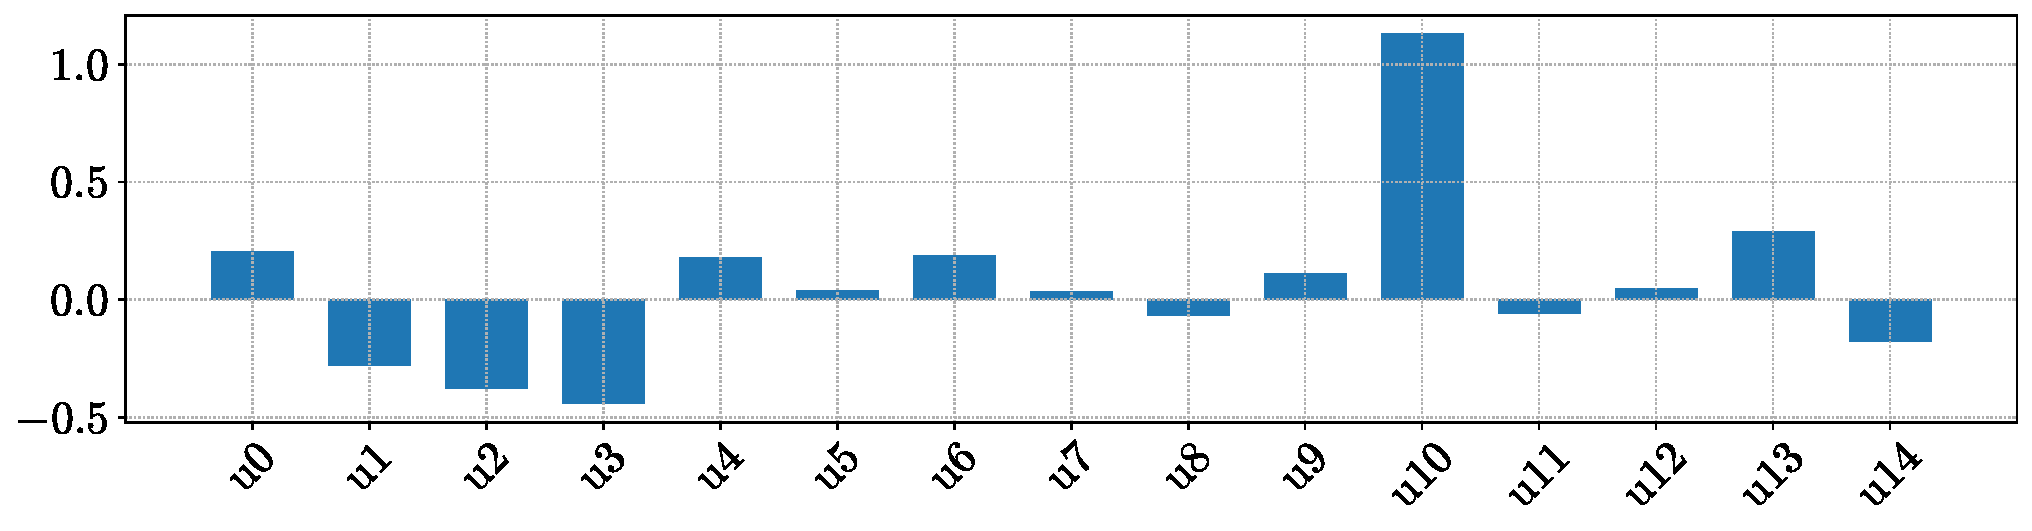
\includegraphics[width=0.85\linewidth]{./img/_biomed_coeff_linear.pdf}
            \caption{Coefficients for this problem}
        \end{figure}

    \item[Issues]
        A linear model has several limitations for explainability:
        \begin{itemize}
            \item Being linear, it might not have good performance on the training data. Therefore, feature analysis might not be accurate.
            \item Only linear correlations can be captured.
            \item Coefficients are not necessarily sparse as L1 has to balance between sparsification and overfitting.
        \end{itemize}
\end{description}

\begin{remark}
    A linear model approach is similar to using the correlation matrix. The only difference is that:
    \begin{itemize}
        \item Pearson's coefficient is computed between a pair of variables.
        \item A linear model considers all the variables at once.
    \end{itemize}
\end{remark}



\subsection{Non-linear model}

\begin{description}
    \item[Non-linear model for explanation] \marginnote{Non-linear model for explanation}
        Use a non-linear model (gradient boosted trees in this case) as a proxy to explain the features.

        \begin{remark}
            Compared to linear models, non-linear models might have better performance but are less explainable and risks overfitting.
        \end{remark}

    \item[Features importance analysis]
        By using trees, feature importances can be computed.

        \begin{figure}[H]
            \centering
            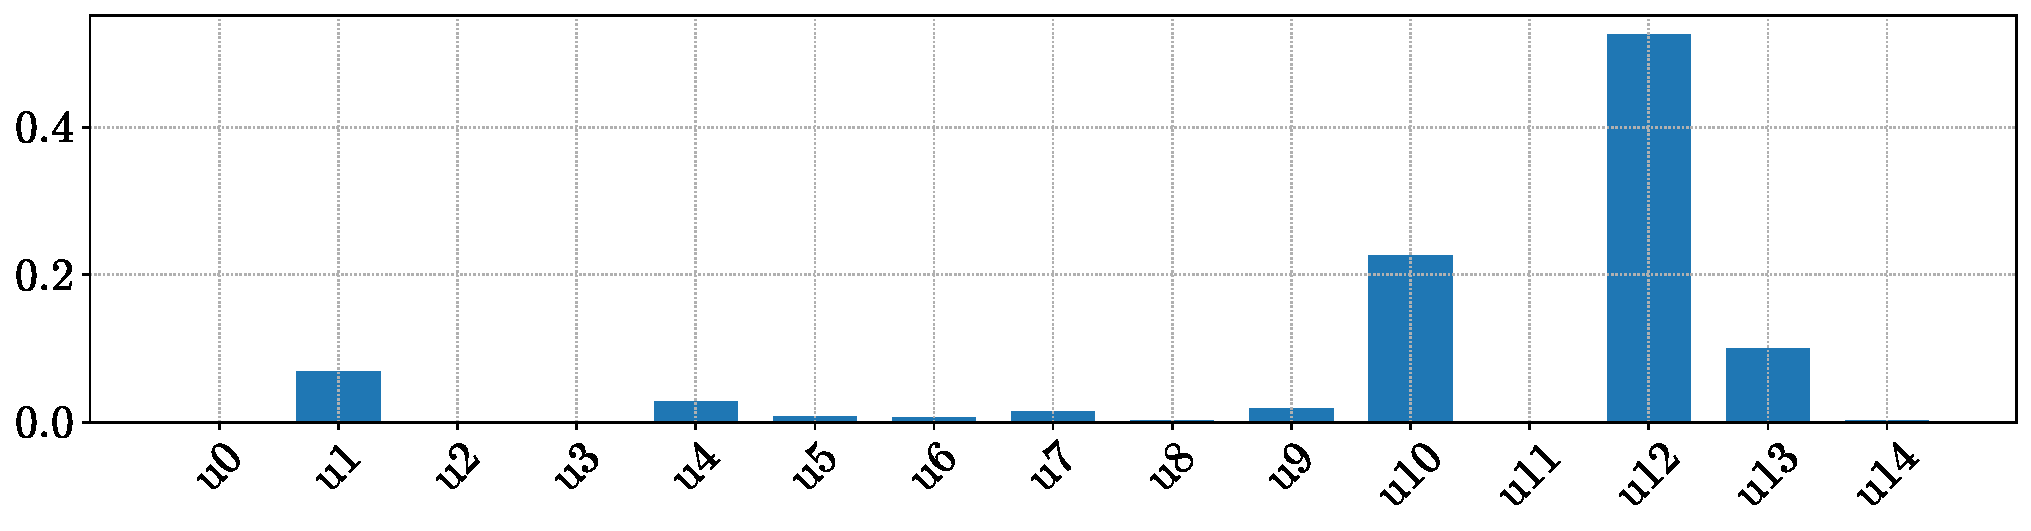
\includegraphics[width=0.85\linewidth]{./img/_biomed_gbt_importance.pdf}
            \caption{Feature importances (gain) for this problem}
        \end{figure}

        \begin{remark}
            Feature importance can be computed using different metrics which will not necessarily produce the same results. Some possible metrics are:
            \begin{descriptionlist}
                \item[Weight] The number of times a feature has been used to split.
                \item[Gain] Average gain from the splits of a feature.
                \item[Cover] Average number of examples for which a feature is used as decision criteria.
                \item[Total gain] Sum of the gains from the splits of a feature.
                \item[Total cover] Sum of the number of examples for which a feature is used as decision criteria.
            \end{descriptionlist}

            \begin{figure}[H]
                \centering
                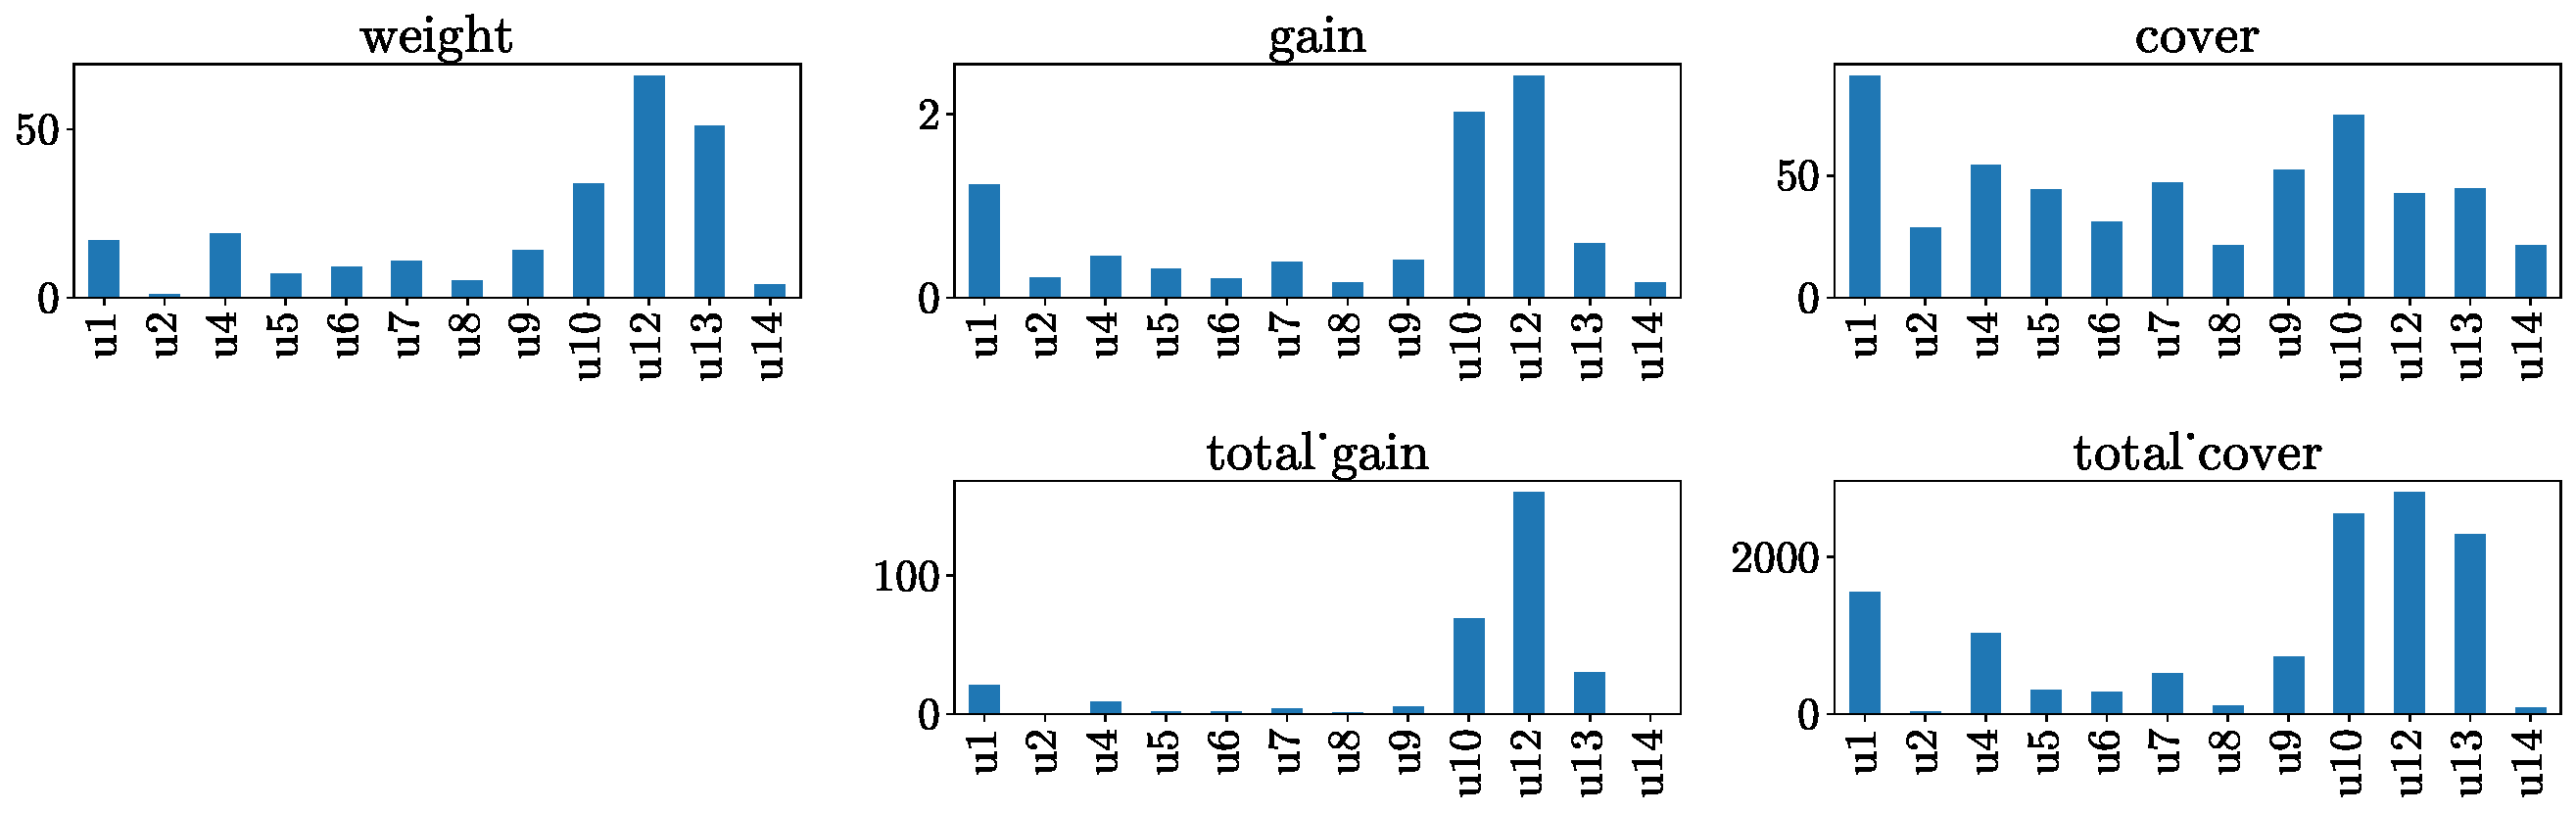
\includegraphics[width=0.95\linewidth]{./img/_biomed_feature_importances_all.pdf}
            \end{figure}

            Moreover, feature importances are associated with the training data. Therefore, it risks overfitting.
        \end{remark}

    \item[Permutation importance analysis] \marginnote{Permutation importance analysis}
        Given:
        \begin{itemize}
            \item A trained model, 
            \item An evaluation metric,
            \item A reference dataset $\{ x_i, y_i \}_{i=1}^m$.
        \end{itemize}
        Permutation importance for the $j$-th feature is computed by randomly permuting the $j$-th column in the dataset and computing the difference between the performance on the original and permuted dataset.

        For more statistical relevance (i.e., remove spurious correlations), the process can be repeated multiple times and presented using mean and standard deviation.

        \begin{remark}
            Permuting the values of a feature aims at preserving the distribution of the column while breaking all correlations.
        \end{remark}

        \begin{remark}
            This approach works on black box models. However, it tends to be expensive.
        \end{remark}

        \begin{remark}
            If the reference dataset is the training set, permutation importance can be used to determine how the model is using the data. On the other hand, by using the test set, the scores will reflect the correlation between the attributes and the target.

            \begin{figure}[H]
                \centering
                \begin{subfigure}{0.8\linewidth}
                    \centering
                    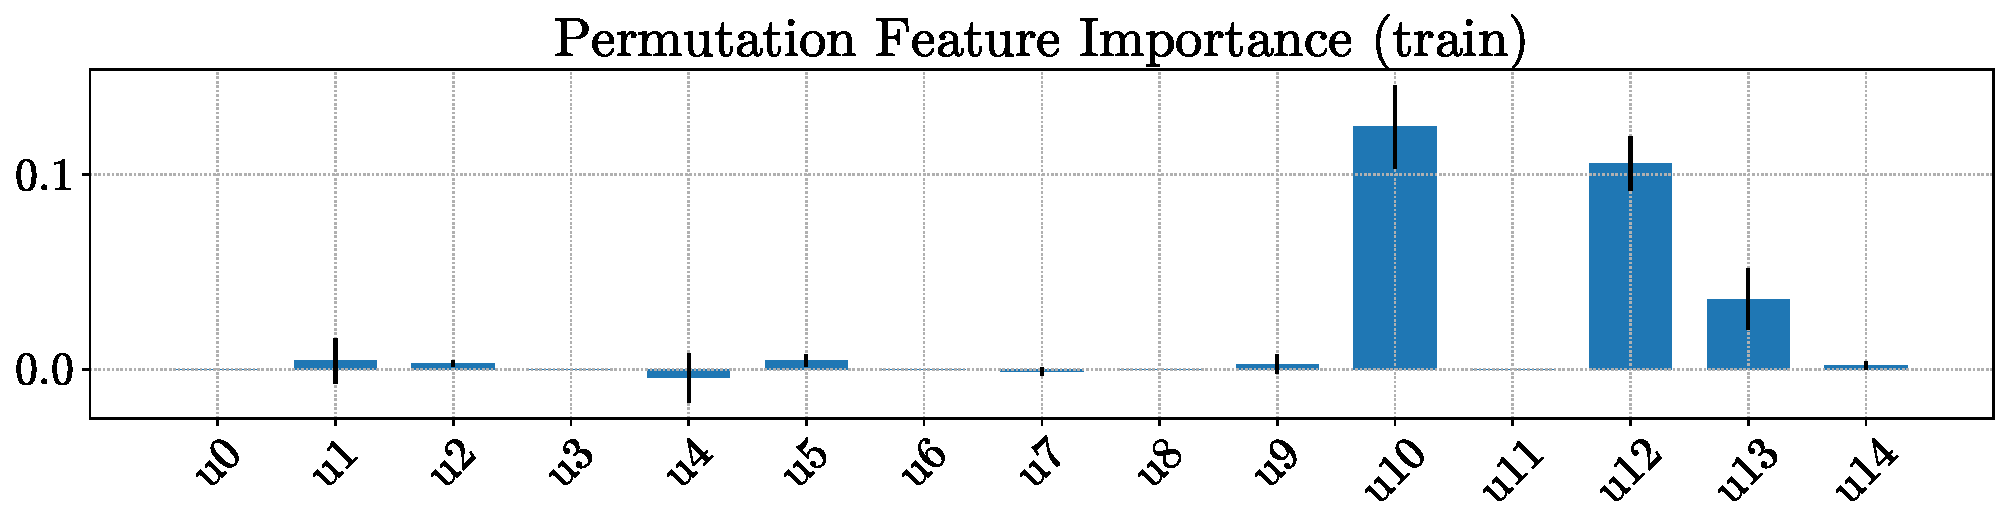
\includegraphics[width=\linewidth]{./img/_biomed_perm_importance_train.pdf}
                \end{subfigure}
                \begin{subfigure}{0.8\linewidth}
                    \centering
                    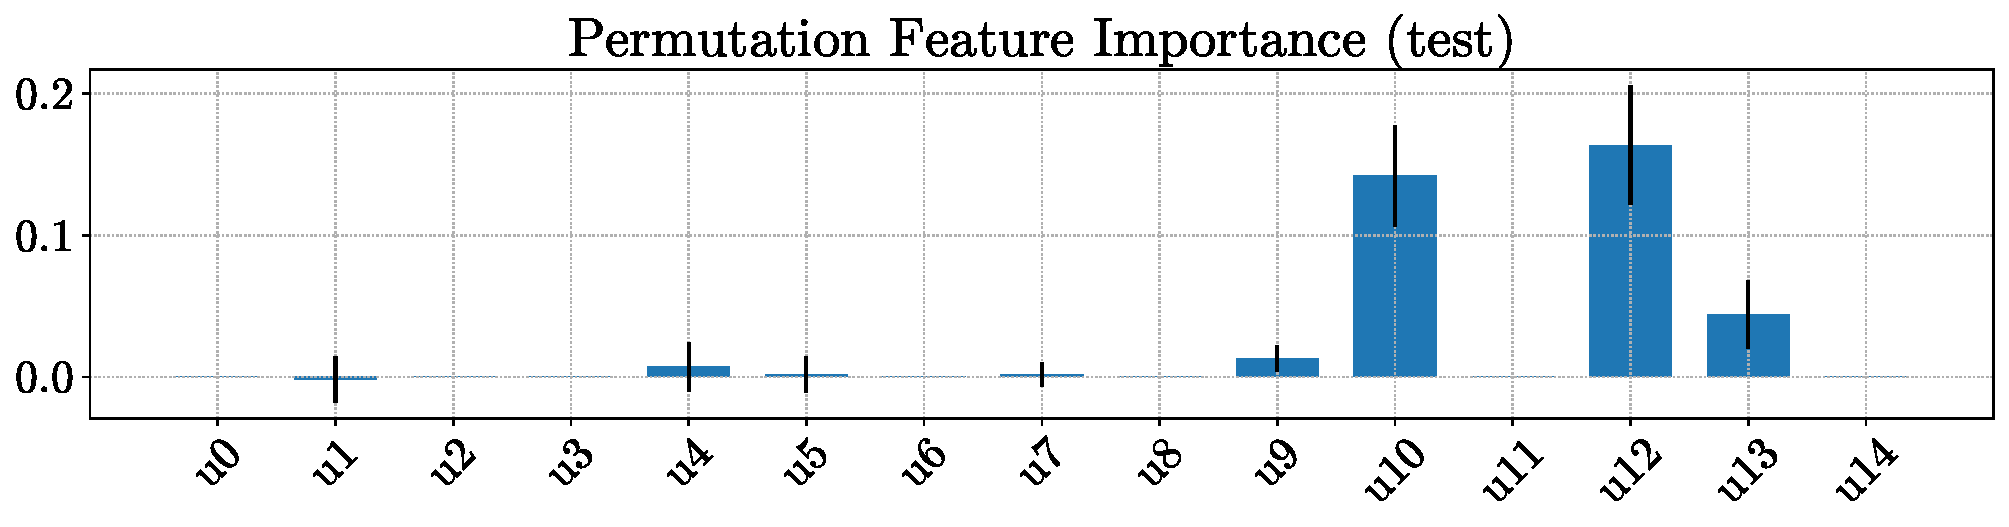
\includegraphics[width=\linewidth]{./img/_biomed_perm_importance_test.pdf}
                \end{subfigure}
                \caption{
                    \parbox[t]{0.7\linewidth}{
                        Permutation importance on train and test set. $u_{10}$ is slightly higher on the train set, which indicates that it might be causing a bit of overfitting.
                    }
                }
            \end{figure}
        \end{remark}
\end{description}

\begin{remark}
    Compared to linear models, non-linear models do not have the capability of identifying the direction of correlation.
\end{remark}


\subsection{Additive feature attribution}

\begin{description}
    \item[Linear models]
        Given a linear model, an individual example $\vec{x}$ can be explained using an additive attribution model as the difference between the prediction and average prediction over the distribution:
        \[ \vec{\theta}^T \vec{x} - \mathbb{E}_{\vec{x}' \in P(\matr{X})}\left[ \vec{\theta}^T \vec{x}' \right] \]
        $\mathbb{E}_{\vec{x}' \in P(X)}\left[ \vec{\theta}^T \vec{x}' \right]$ can be approximated as the average prediction on the training data and it represents the prediction that the model would make if no information is provided.

        Due to linearity, the formula can be rewritten as follows:
        \[ 
            \begin{split}
                \vec{\theta}^T \vec{x} - \mathbb{E}_{\vec{x}' \in P(\matr{X})}\left[ \vec{\theta}^T \vec{x}' \right] &= \vec{\theta}^T(\vec{x} - \mathbb{E}_{\vec{x}' \in P(\matr{X})}\left[ \vec{x}' \right]) \\
                &= \sum_{j=1}^{n} \vec{\theta}_j (\vec{x}_j - \mathbb{E}_{\vec{x}' \in P(\matr{X})}\left[ \vec{x}'_j \right]) \\
                &= \sum_{j=1}^{n} \phi_j(\vec{x})
            \end{split}
        \]
        where $\phi_j(\vec{x}) = \vec{\theta}_j (\vec{x}_j - \mathbb{E}_{\vec{x}' \in P(\matr{X})}[\vec{x}'_j])$ is the \textbf{effect}\marginnote{Effect} of the $j$-th attribute on the output for the example $\vec{x}$ (i.e., how much it moves from the baseline prediction).

    \item[Non-linear models]
        Given a non-linear model, an example $\vec{x}$ can be explained using an additive attribution model defined as follows:
        \[ g(\vec{z}, \vec{x}) = \phi_0 + \sum_{j=1}^{n} \phi_j(\vec{x}) \vec{z}_j \]
        where:
        \begin{itemize}
            \item $\phi_0$ is the baseline prediction (i.e., average prediction over the dataset).
            \item $\phi_j$ is the effect of the $j$-th feature.
            \item $\vec{z}_j \in \{ 0, 1 \}$ indicates whether the $j$-th feature is known.
        \end{itemize}

        In practice, given an example $\vec{x}$ and the flags $\vec{z}$, a linear explanation model is trained locally to tune the effect coefficients $\phi_j$ of $g(\vec{z}, \vec{x})$.

        \begin{description}
            \item[Shapely values] \marginnote{Shapely values}
                Closed-form formula to determine the effect coefficients. Given the set of all input features $\mathcal{J}$, the Shapely value of the $j$-th feature is computed as:
                \[ \phi_j(\vec{x}) = \sum_{\mathcal{S} \subset \mathcal{J} \smallsetminus j} \frac{|\mathcal{S}|! (n - |\mathcal{S}| - 1)!}{n!} (\hat{f}(\vec{x}_{\mathcal{S} \cup j}) - \hat{f}(\vec{x}_{\mathcal{S}})) \]
                Intuitively, by fixing the $j$-th attribute, $\phi_j$ is computed by considering all the possible combinations of the $\vec{z}_i$ values of the other attributes (i.e., different subsets $\mathcal{S}$ of the features without $j$) and averaging the difference between the prediction that uses as features $\mathcal{S} \cup j$ and the baseline that only uses $\mathcal{S}$.

                \begin{remark}
                    Shapely values are expensive to compute due to the exponential number of terms. Moreover, many models do not support missing values.
                \end{remark}
        \end{description}

    \item[SHAP] \marginnote{SHAP}
        Framework to approximate Shapely values for black-box models.

        \begin{description}
            \item[Kernel SHAP] 
                Given an example $\vec{x}$, kernel SHAP does the following:
                \begin{enumerate}
                    \item Sample multiple $\vec{z}'$ vectors from $\{ 0, 1 \}^n$.
                    \item For every sampled vector, construct an example $\vec{x}'$ such that:
                    \begin{itemize}
                        \item $\vec{x}'_j = \vec{x}_j$ if $\vec{z}'_j = 1$.
                        \item $\vec{x}'_j$ is sampled from a background set (e.g., training set) if $\vec{z}'_j = 0$.
                    \end{itemize}
                    \item Train a linear model on the created examples and determine Shapely values using it.
                \end{enumerate}

                \item[Plots]
                    Shapely values can be visualized through several plots:

                    \begin{description}
                        \item[Waterfall plot] 
                            Shows the most relevant features that allowed to reach the prediction $f(x)$ starting from the baseline $\mathbb{E}[f(x)]$.
                            \begin{figure}[H]
                                \centering
                                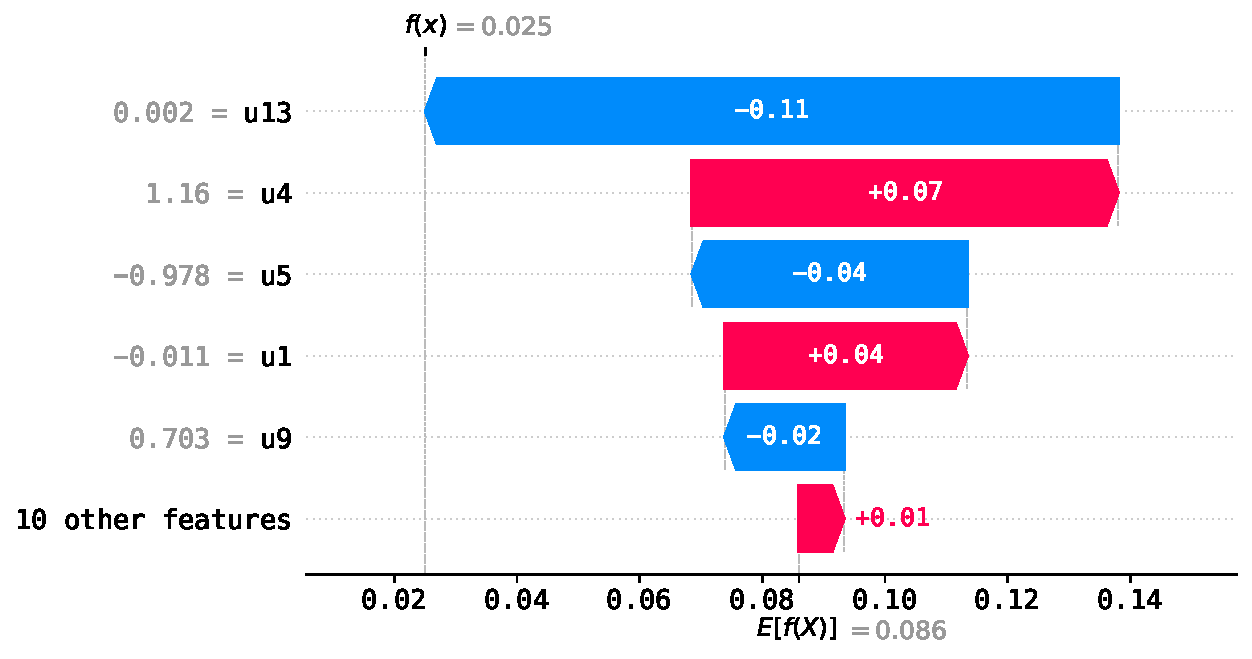
\includegraphics[width=0.6\linewidth]{./img/_biomed_shap_waterfall.pdf}
                            \end{figure}

                        \item[Force plot] 
                            Compact version of waterfall plots.
                            \begin{figure}[H]
                                \raggedleft
                                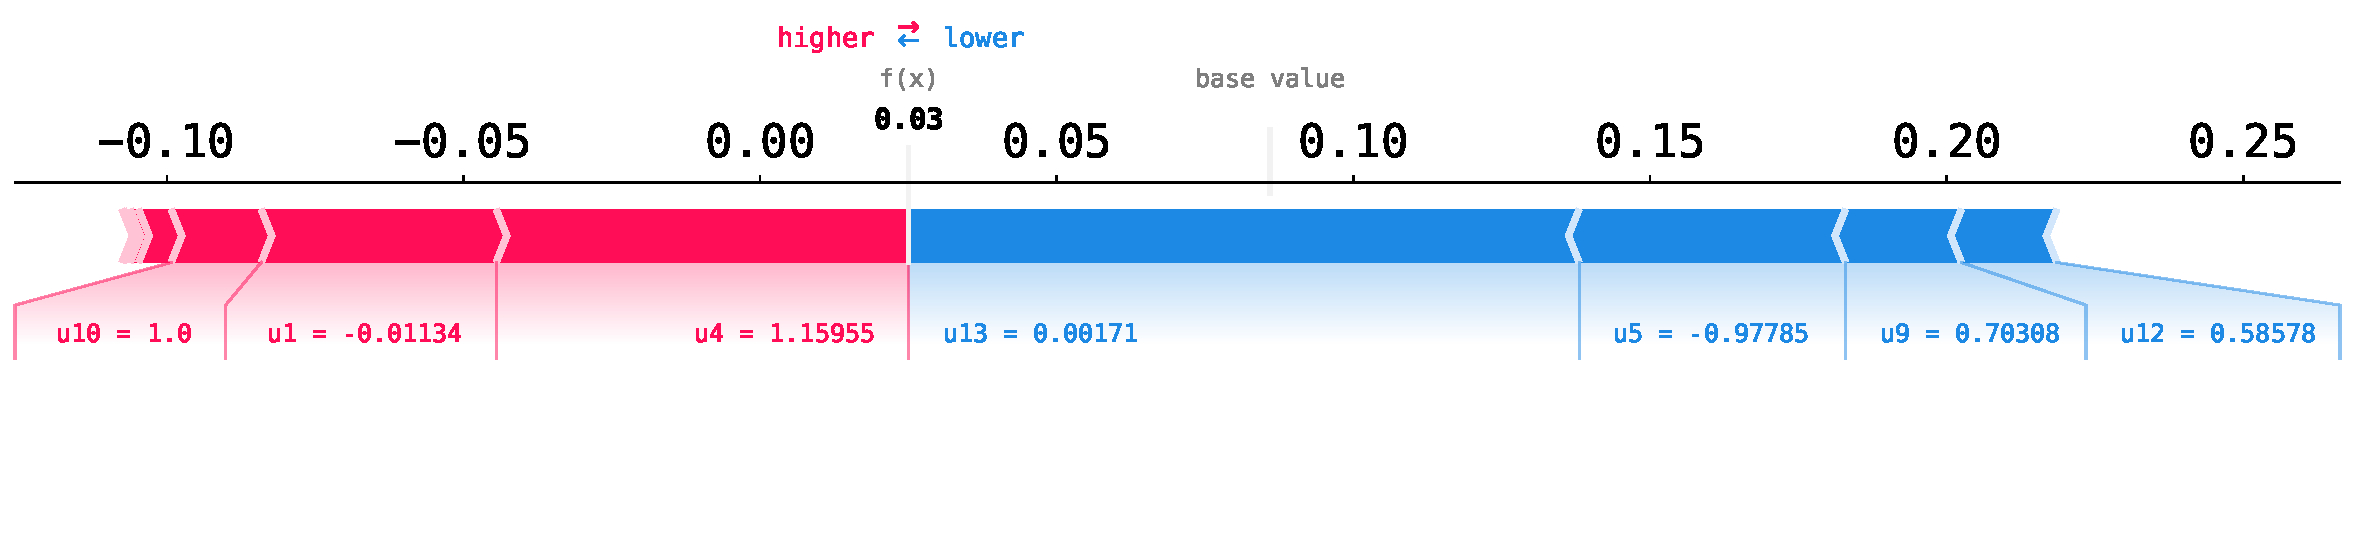
\includegraphics[width=0.8\linewidth]{./img/_biomed_shap_force.pdf}
                            \end{figure}

                        \item[Global force plot] 
                            Stack of force plots where the $x$-axis represents the examples.
                            \begin{figure}[H]
                                \raggedleft
                                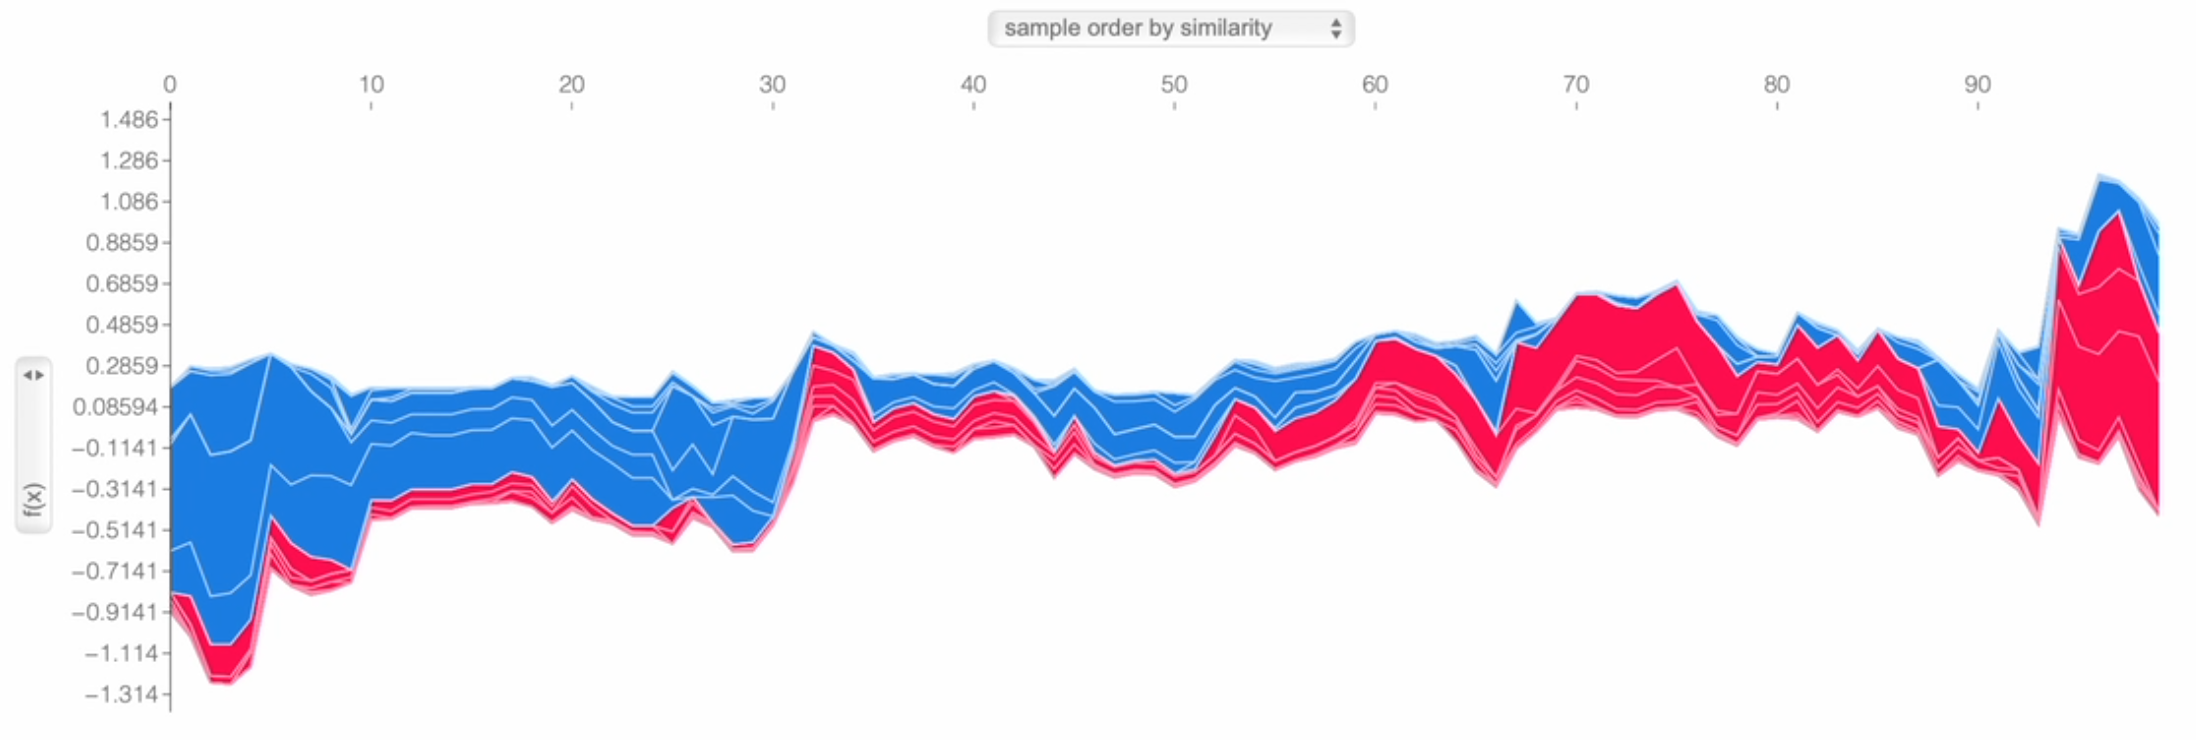
\includegraphics[width=0.8\linewidth]{./img/biomed_shap_global_force.png}
                            \end{figure}

                        \item[Scatter plot] 
                            Links the values of an attribute to its Shapely values.
                            \begin{figure}[H]
                                \raggedleft
                                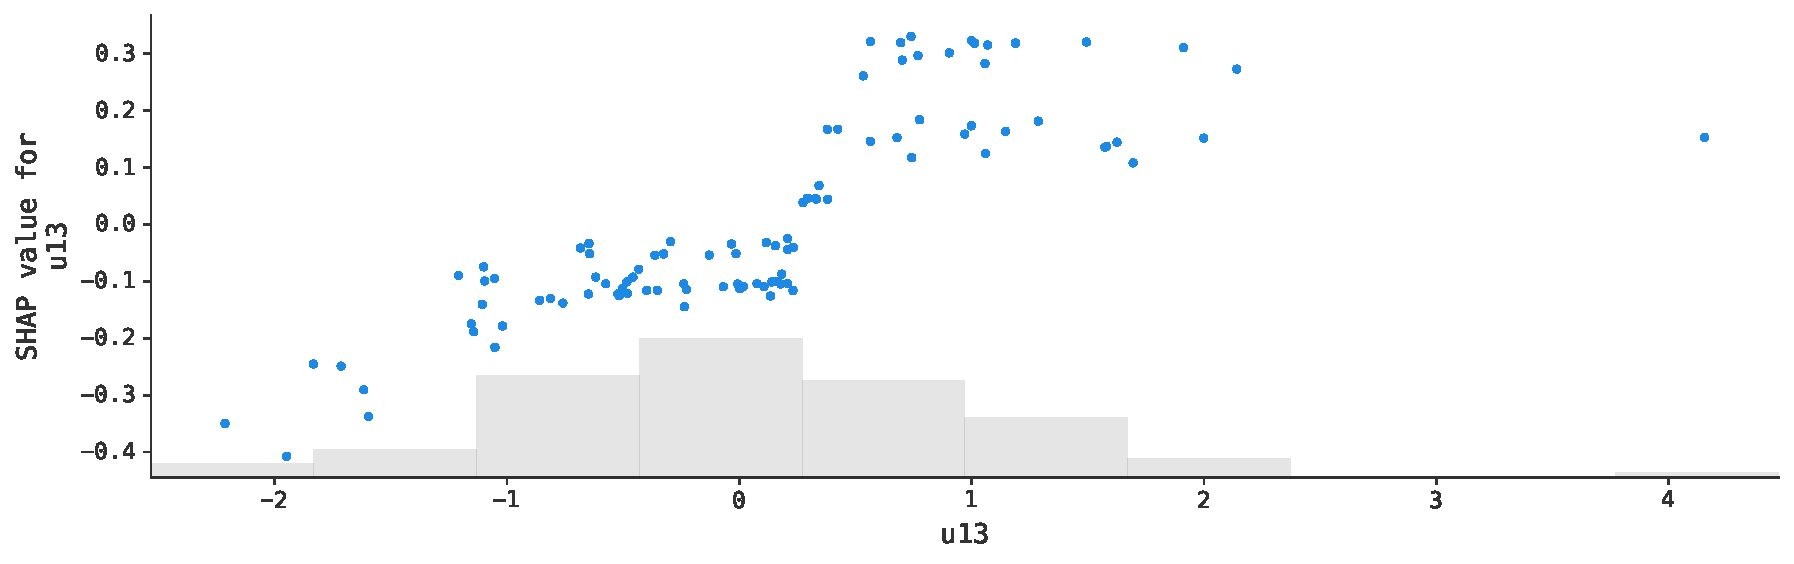
\includegraphics[width=0.8\linewidth]{./img/_biomed_shap_scatter.pdf}
                            \end{figure}

                            \begin{remark}
                                A growing trend indicates a positive correlation.
                            \end{remark}

                        \item[Beeswarm summary plot] 
                            Stack of multiple scatter plots. The values of the attributes are color coded (instead of being at the $x$-axis).
                            \begin{figure}[H]
                                \raggedleft
                                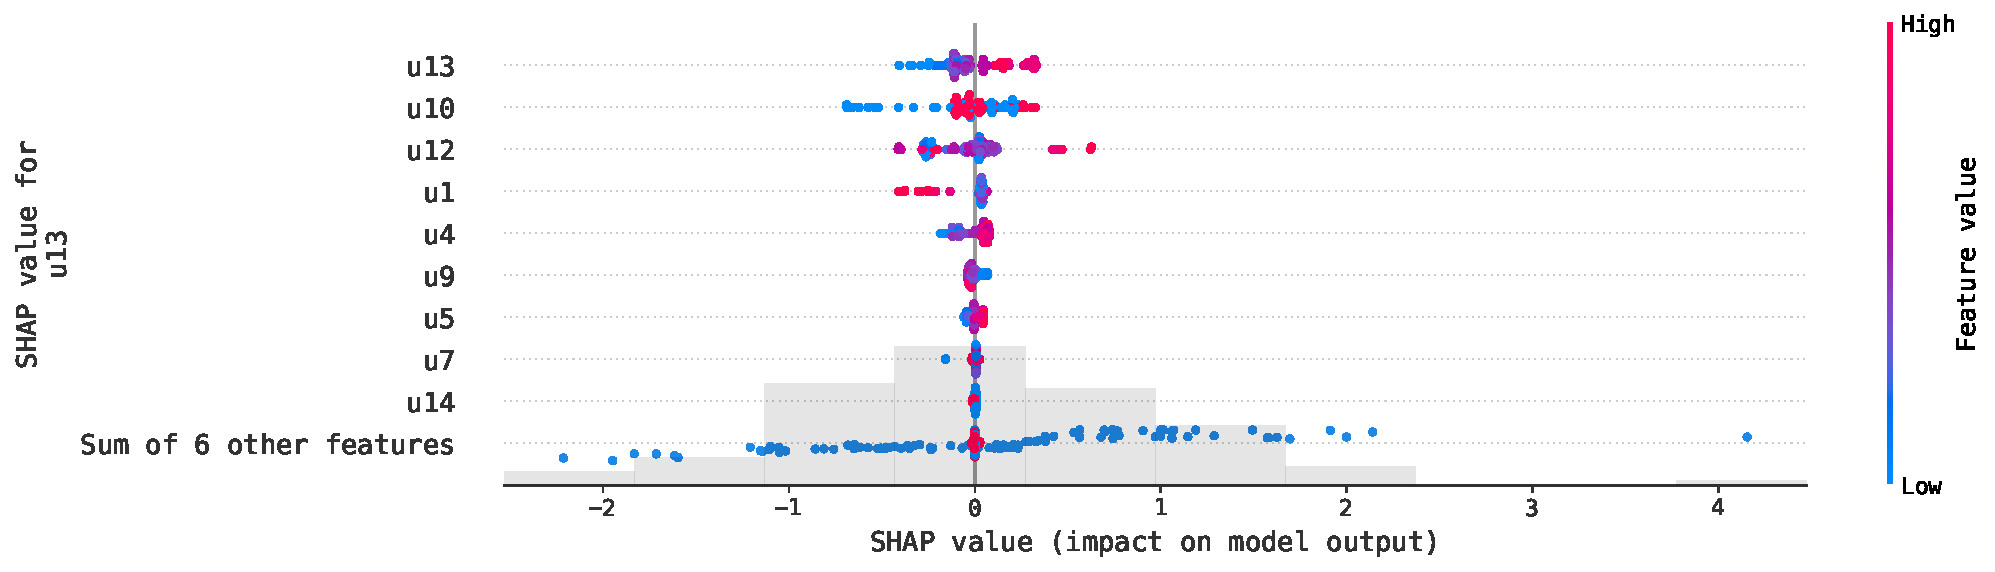
\includegraphics[width=0.8\linewidth]{./img/_biomed_shap_beeswarm.pdf}
                            \end{figure}

                            \begin{remark}
                                A color gradient indicates correlation.
                            \end{remark}

                        \item[Scatter dependency plot] 
                            Links the combined effect of two attributes. Starting from the scatter plot of the first attribute, points are colored based on the values of the second attribute.
                            \begin{figure}[H]
                                \raggedleft
                                \begin{subfigure}{0.8\linewidth}
                                    \raggedleft
                                    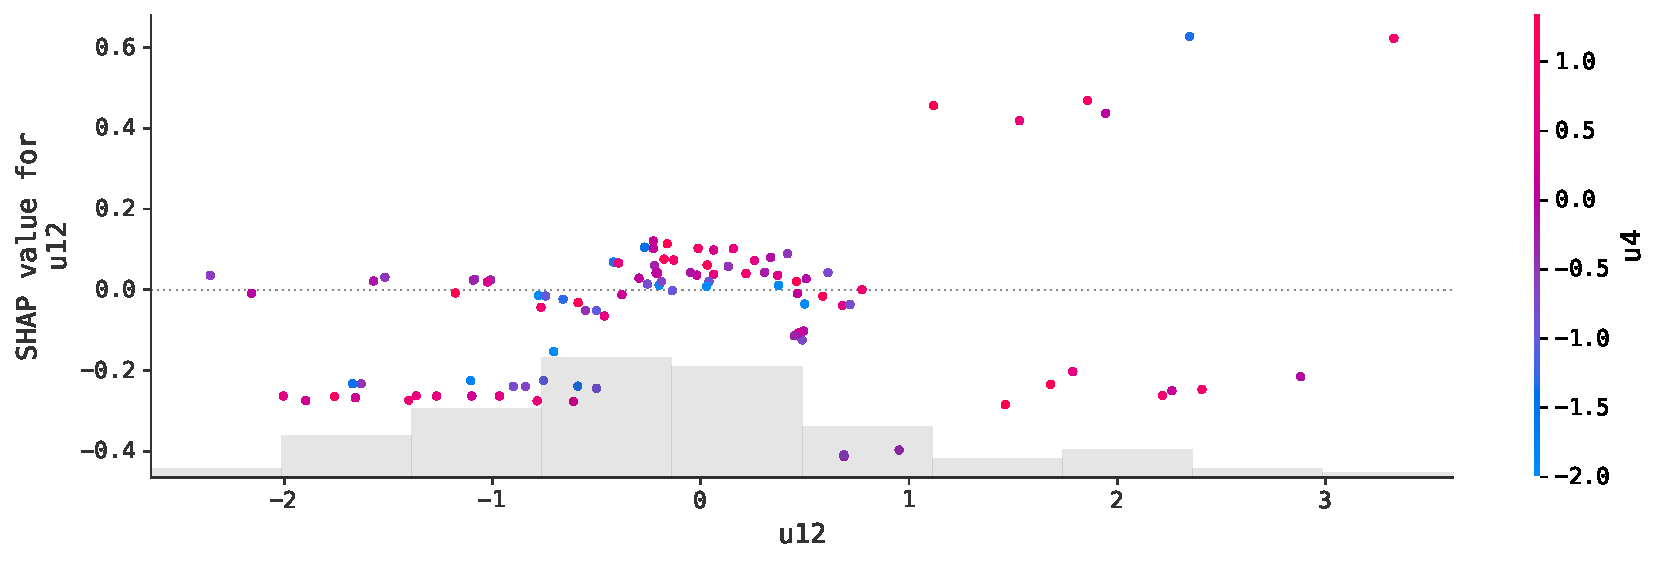
\includegraphics[width=\linewidth]{./img/_biomed_shap_dependecy1.pdf}
                                \end{subfigure}
                                \begin{subfigure}{0.8\linewidth}
                                    \raggedleft
                                    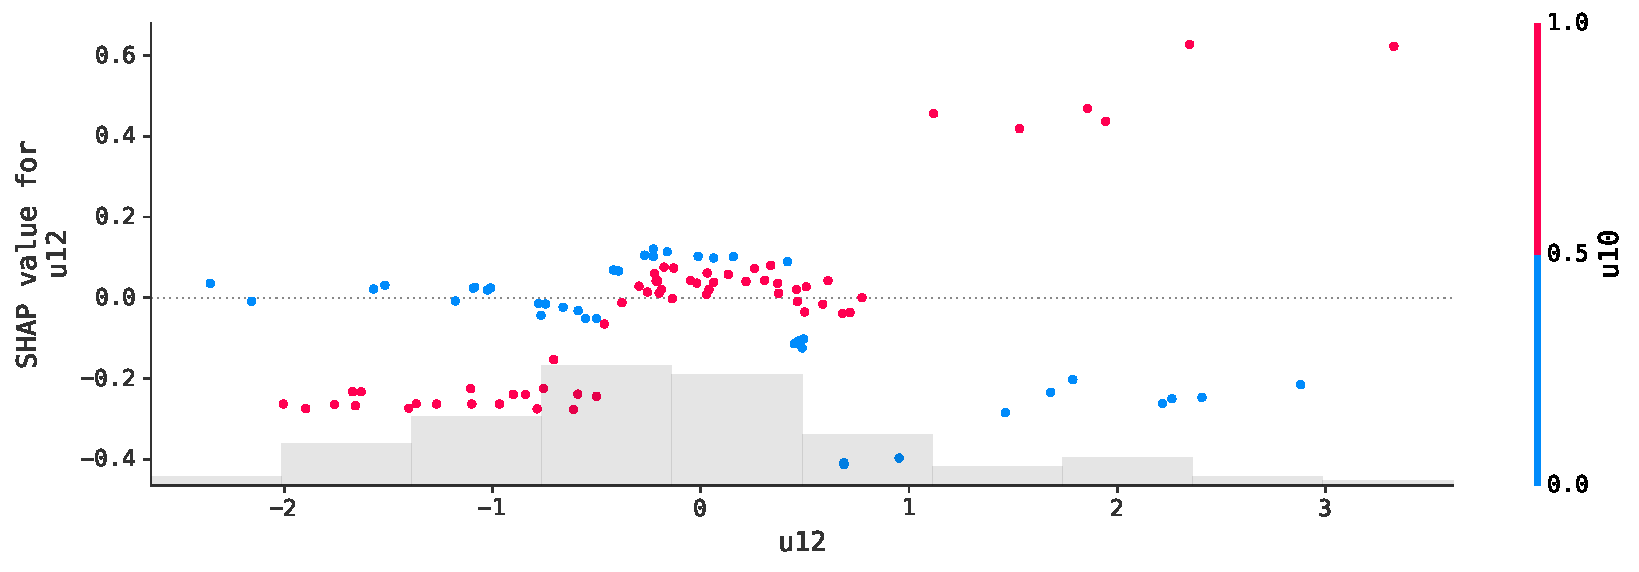
\includegraphics[width=\linewidth]{./img/_biomed_shap_dependency2.pdf}
                                \end{subfigure}
                            \end{figure}
                    \end{description}
        \end{description}

        \begin{remark}
            As is, SHAP does not provide single values (e.g., feature importance) but only values for each example.
        \end{remark}

        \begin{description}
            \item[Global feature analysis]
                Aggregate local Shapely values to obtain global explanations. For instance, a possible approach is averaging over the examples:
                \[ \bar{\phi}_j(x) = \frac{1}{n} \sum_{i=1}^{m} | \phi_j(x_i) | \]

                \begin{remark}
                    This approach is heuristic. Shapely values have well-defined semantics and the result of aggregation is not clear.
                \end{remark}

                \begin{figure}[H]
                    \centering
                    \begin{subfigure}{0.48\linewidth}
                        \centering
                        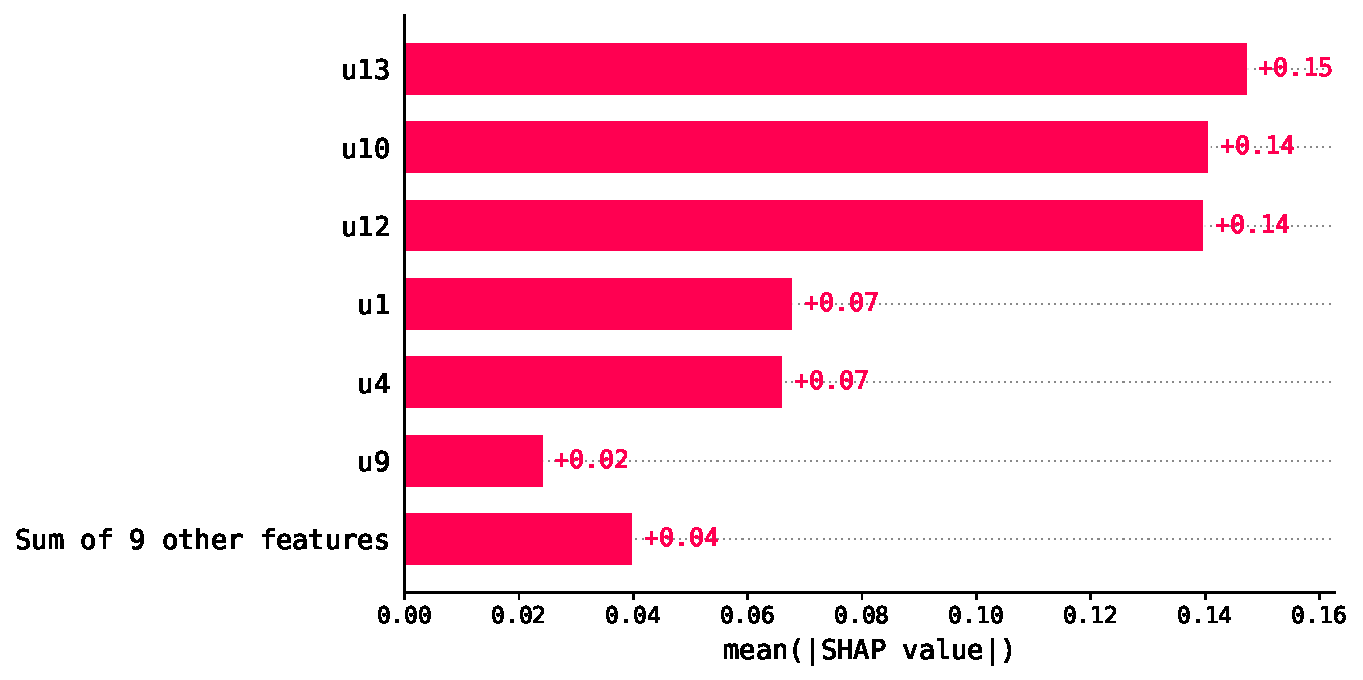
\includegraphics[width=\linewidth]{./img/_biomed_shap_aggr_avg.pdf}
                    \end{subfigure}
                    \begin{subfigure}{0.48\linewidth}
                        \centering
                        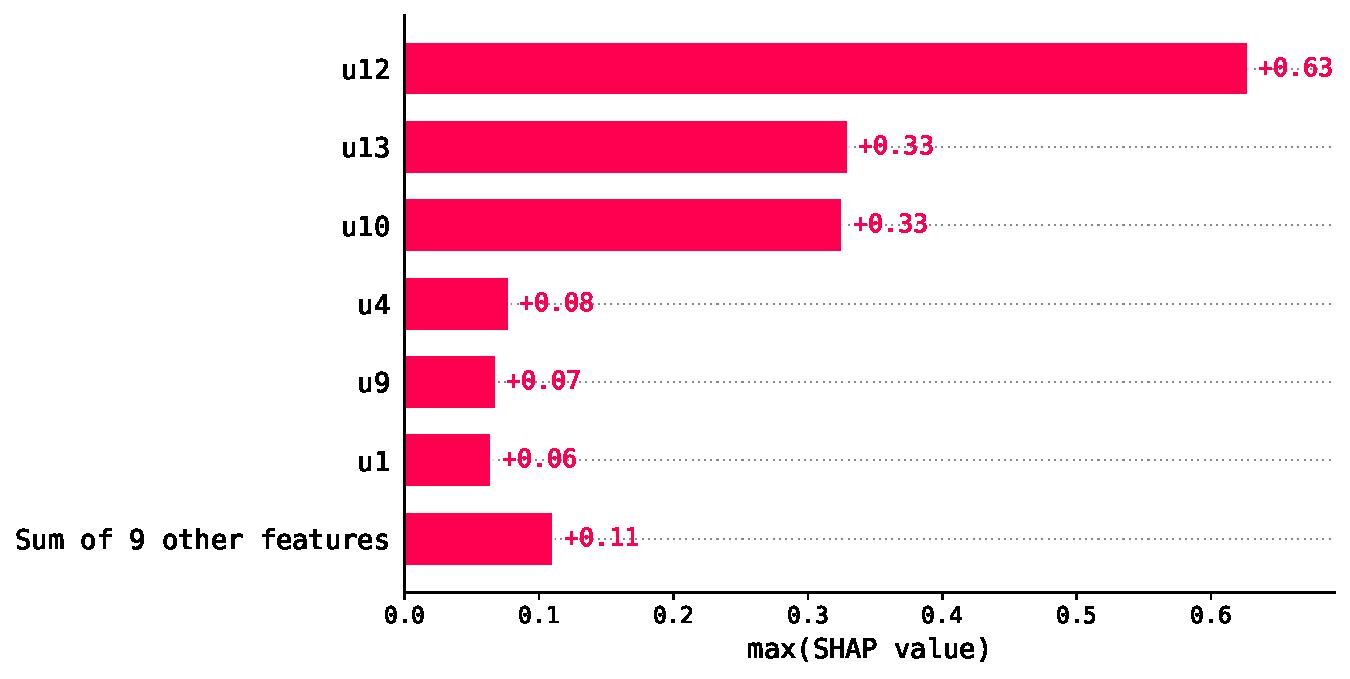
\includegraphics[width=\linewidth]{./img/_biomed_shap_aggr_max.pdf}
                    \end{subfigure}
                \end{figure}
        \end{description}
\end{description}


\subsection{Optimization-oriented feature selection}

\begin{description}
    \item[Optimization-oriented feature selection] \marginnote{Optimization-oriented feature selection}
        Given the set of features $\mathcal{J}$, solve the problem:
        \[ \arg\min_{\mathcal{S} \subseteq \mathcal{J}} \left\{ |\mathcal{S}|: \forall (x, y).\, \hat{y} = \hat{f}_\mathcal{S}(x_\mathcal{S}), \mathcal{L}(y, \hat{y}) \leq \theta \right\} \]
        In other words, this is the problem of determining the smallest subset of features $\mathcal{S}$ such that a model $\hat{f}_\mathcal{S}$ trained only considering them has an acceptable performance.

        \begin{remark}[Pareto fronts]
            This problem can be solved as a multi-objective optimization problem using Pareto fronts to discard unnecessary points and only consider those that graphically do not have other points in the top-left area above them.

            \begin{figure}[H]
                \centering
                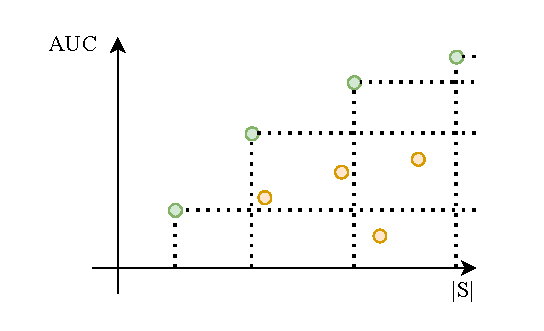
\includegraphics[width=0.5\linewidth]{./img/_pareto_front.pdf}
                \caption{Green points are non-dominated and orange points are dominated}
            \end{figure}
        \end{remark}

        \begin{remark}
            This approach aims at obtaining the best possible performance. Therefore, it is reasonable for a normal machine learning problem. However, for determining features importance, this is not ideal.
        \end{remark}
\end{description}


\subsection{Statistical hypothesis testing}

\begin{description}
    \item[Statistical hypothesis testing] \marginnote{Statistical hypothesis testing}
        Given:
        \begin{itemize}
            \item A random (possibly multivariate) variable $X$,
            \item A hypothesis $H(X)$.
        \end{itemize}
        We can define:
        \begin{itemize}
            \item A competing null hypothesis $H_0(X)$,
            \item An experimental statistics $T[X]$ (e.g., expected value).
        \end{itemize} 

        \begin{remark}
            $H_0$ is often the negation of $H$ and $T[X]$ is a value that supports the hypothesis when large enough.
        \end{remark}

        By assuming that the null hypothesis holds, we need to compute:
        \begin{itemize}
            \item The empirical value $T[x \mid H_0]$.
            \item The theoretical probability $\prob{T[X \mid H_0]}$.
        \end{itemize}

        \begin{description}
            \item[$p$-value] \marginnote{$p$-value} 
                Probability $\prob{T[X \mid H_0]}$ of observing an empirical value as extreme as $\prob{T[X]}$ under the null hypothesis (e.g., $\prob{T[X \mid H_0] \geq t}$ or  $\prob{T[X \mid H_0] \leq t}$, depending on the case). If $p < 1-\alpha$, for a given confidence interval $\alpha$ (e.g., $0.95$), $H_0$ is likely false.
        \end{description}
\end{description}

\begin{example}
    For this problem:
    \begin{itemize}
        \item Variables can be feature-target pairs $(X, Y)$.
        \item The hypothesis can be $H \equiv \text{``$X$ is important to predict $Y$''}$ (following a given correlation score $r[X, Y]$ such as average Shapely value, permutation importance, \dots).
        \item The null hypothesis can be $H_0 \equiv \text{``X is important by chance''}$.
    \end{itemize}

    Given the correlation score for the original dataset $r^* = r[x, y]$, we can define the following inequality:
    \[ r[\tilde{x}, \tilde{y}] \leq r^* \]
    where $(\tilde{x}, \tilde{y})$ is sampled from $(\tilde{X}, \tilde{Y})$, which is a similar but uncorrelated version of $(X, Y)$. If $X$ and $Y$ are correlated, it is expected that the inequality holds most of the time, otherwise it should be half of the time. Therefore, we can define the test statistics for this problem as:
    \[ T[X, Y \mid H_0] \equiv \sum_{i=1}^{m} \prob{r[\tilde{X}, \tilde{Y}] \leq r^*} \]
    where $m$ is the number of samples drawn from $(\tilde{X}, \tilde{Y})$. If $T[X, Y \mid H_0] \sim \frac{m}{2}$, we can state that $X$ and $Y$ might not be correlated.

    The test $r[\tilde{X}, \tilde{Y}] \leq r^*$ has a binary outcome and therefore its theoretical probability follows a Bernoulli distribution (if $H_0$ holds, it follows $\mathcal{B}(\frac{1}{2})$). If the experiment is repeated $n$ times, the probability of $T[X, Y \mid H_0]$ follows a binomial distribution $\mathcal{B}(n, \frac{1}{2})$.

    In practice, to create an uncorrelated dataset $(\tilde{X}, \tilde{Y})$, it is possible to permute the values of a feature in $X$. Then, it is possible to compute the empirical value $T[X, Y \mid H_0]$ and match it against the theoretical probability. The $p$-value can be computed as:
    \[ p = \prob{T[X, Y \mid H_0] \geq t} \]
    where $t$ defines a target interval in the distribution and depends on the theoretical distribution and the confidence level $\alpha$. If $p < 1-\alpha$, we can reject $H_0$. To reduce sampling noise, the experiment can be repeated multiple times.

    \begin{figure}[H]
        \centering
        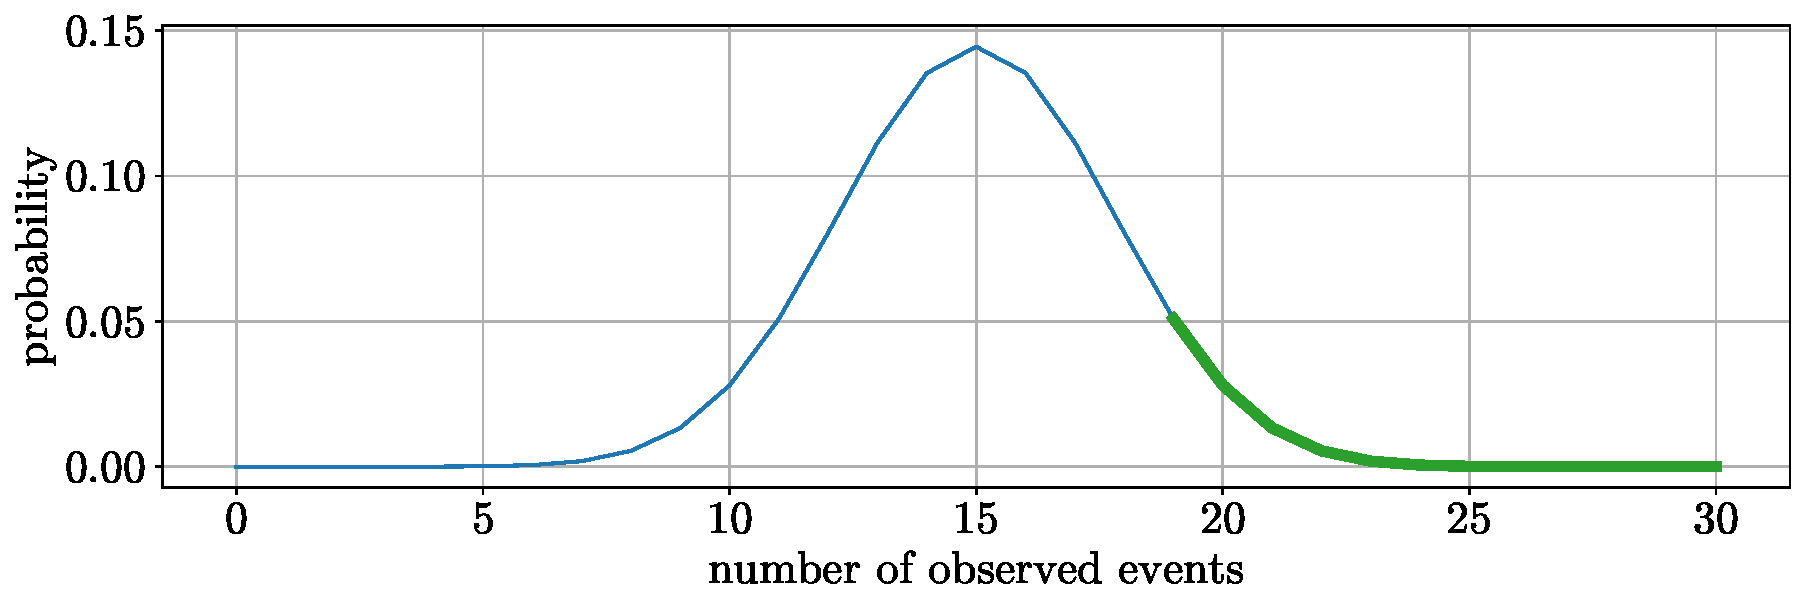
\includegraphics[width=0.6\linewidth]{./img/_biomed_pvalue.pdf}
        \caption{
            \parbox[t]{0.5\linewidth}{
                Binomial distribution with 30 samples. The interval defined with $\alpha=0.95$ is in green.
            }
        }
    \end{figure}
\end{example}

\begin{remark}
    When $p < 1-\alpha$, it is possible to reject $H_0$ and state that $H$ is most likely true. However, in all other cases nothing can be concluded. 

    With binary hypotheses, it is possible to negate $H$ and repeat the procedure with $\lnot H$, allowing to create two target intervals to have more information.
\end{remark}

\begin{example}
    For this case, we have that:
    \begin{itemize}
        \item The negated hypothesis is $\lnot H \equiv$ ``$X$ is not important to predict $Y$''.
        \item $H_0$ remains the same.
        \item The test statistics becomes $n - T[X, Y \mid H_0]$.
    \end{itemize}
    
    By proceeding as before, we can ultimately obtain the following intervals:
    \begin{itemize}
        \item One that supports $H$.
        \item One that supports $\lnot H$.
        \item One where no claim can be made.
    \end{itemize}

    \begin{figure}[H]
        \centering
        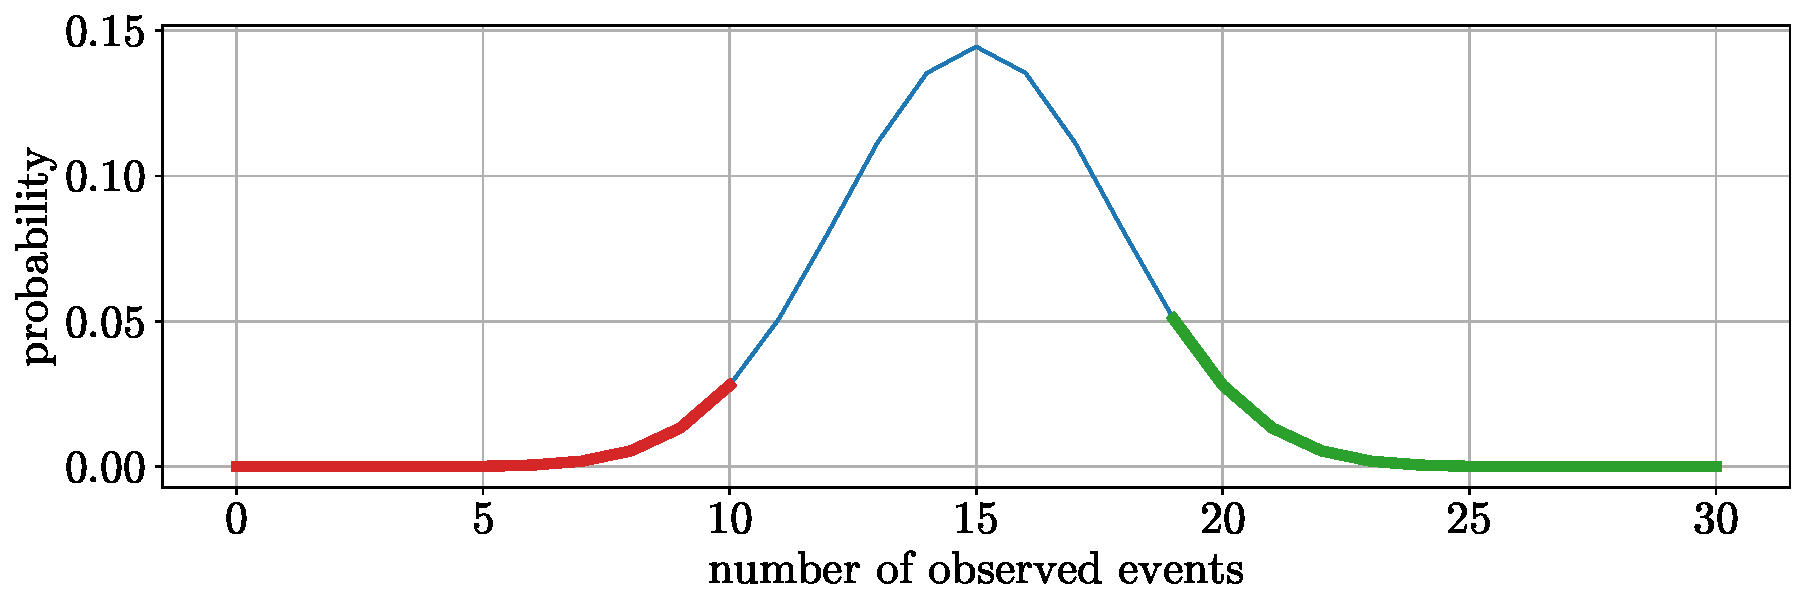
\includegraphics[width=0.6\linewidth]{./img/_biomed_pvalue_two_tails.pdf}
    \end{figure}
\end{example}


\begin{description}
    \item[Boruta] \marginnote{Boruta}
        Algorithm for feature selection based on statistical hypothesis testing with the hypothesis $H \equiv$ ``feature $j$ is important among those in the dataset according to a given metric''

        Given a dataset $(X, Y)$, Boruta works as follows:
        \begin{enumerate}
            \item Augment the dataset with a permuted version $\tilde{X}_j$ of each feature (shadow features).
            \item Run the statistical test based on:
            \[ \phi_j((x, \tilde{x}), y) > \max_{j \in \tilde{X}} \phi_j((x, \tilde{x}), y) \]
            where $\phi$ is a feature importance metric (e.g., obtained from decision trees). Intuitively, the importance of a feature $j$ is compared with the importances of the shadow features.
            \item Repeat the experiment multiple times.
        \end{enumerate}

        \begin{remark}
            Due to the maximum operation, the theoretical distribution of $T$ is mostly binomial. So, some statistical corrections are applied.
        \end{remark}

        \begin{remark}
            Boruta tests both positive and negative hypothesis. Therefore, it is able to determine whether a feature is important, unimportant, or be undecided.
        \end{remark}
\end{description}


\subsection{Ground-truth check}

The synthetic dataset used in this section is described by the following causal graph:
\begin{figure}[H]
    \centering
    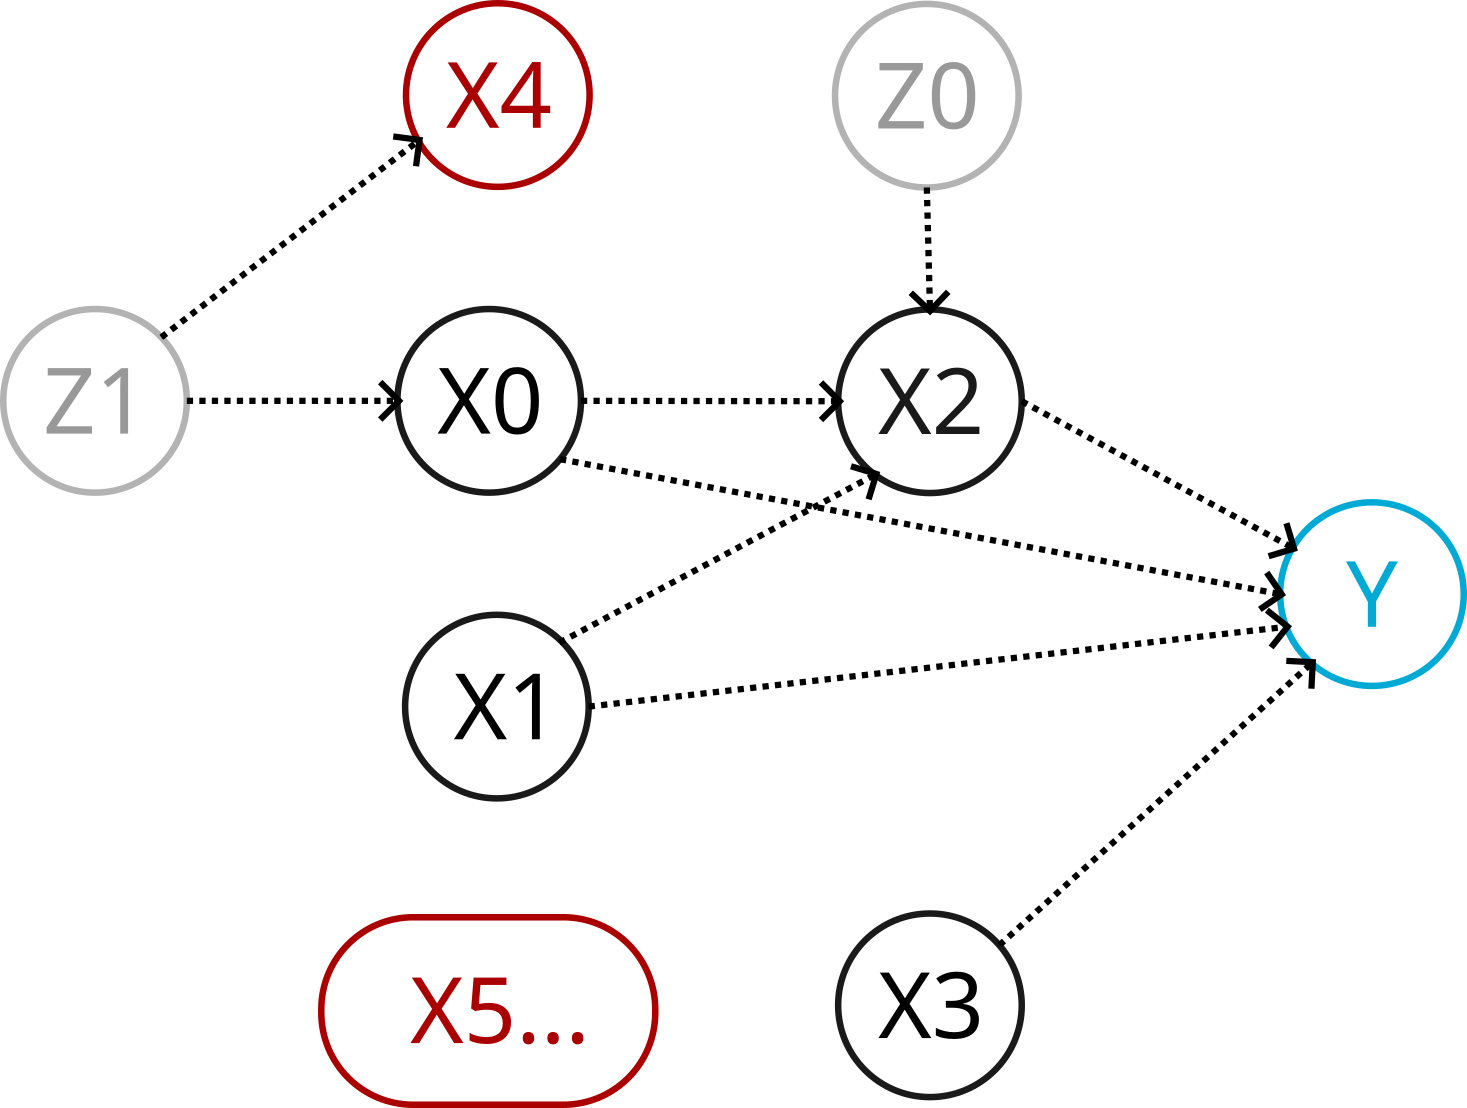
\includegraphics[width=0.3\linewidth]{./img/biomed_causal_graph.png}
\end{figure}
where:
\begin{itemize}
    \item Black variables are relevant for the target.
    \item Gray variables are latent.
    \item Red variables are irrelevant.
\end{itemize}

This graph has some common patterns:
\begin{descriptionlist}
    \item[Mediator] 
        A variable $A$ that hides the effect of another variable $B$. If $A$ affects the target, then $B$ also does.

    \begin{example}
        In the causal graph, $X_2$ is a mediator between $X_0$, $X_1$ and $Y$, which might cause problems to detect $X_0$ and $X_1$ as relevant features. $X_2$ also mediates for $Z_0$, which, in this case, has a positive effect as $Z_0$ is not observed.
    \end{example}

    \begin{remark}
        Strongly correlated features (e.g., mediator-mediator) might mislead algorithms when determining relevant features as a model might partition the importance between the two features.
    \end{remark}

    \item[Confounder]
        A variable $A$ that has effect on two variables $B_1$ and $B_2$. Therefore, it correlates $B_1$ and $B_2$. This might cause to mistakenly consider a variable important for predicting the target.

        \begin{example}
            In the causal graph, $Z_1$ causes a confounder between $X_0$ and $X_4$. $X_4$ might be considered a relevant feature.
        \end{example}
\end{descriptionlist}

Overall, Boruta is able to: 
\begin{itemize}
    \item Identity all causal variables.
    \item Correctly estimate the distribution of almost all the variables.
    \item Determine monotonic effects and mediators.
\end{itemize}